\documentclass[12pt,a4paper]{article}
\PassOptionsToPackage{hidelinks}{hyperref}
\usepackage{ihedn-report}
\addbibresource{bibliographies/bib/rapport.bib}

\usepackage[acronym,toc,section=section]{glossaries}
\makeglossaries
% ---------- Acronymes ----------
\newacronym{codir}{CODIR}{Comité de direction}
\newacronym{dreal}{DREAL}{Direction régionale de l'environnement, de l'aménagement et du logement}
\newacronym[
    plural=DMD,
    longplural=Délégués Militaires Départementaux
]{dmd}{DMD}{Délégué Militaire Départemental}
\newacronym{retex}{RETEX}{Retour d'expérience}
\newacronym{orsec}{ORSEC}{Organisation de la Réponse de SEcurité Civile}
\newacronym{pics}{PICS}{Plans intercommunaux de sauvegarde}
\newacronym{pcs}{PCS}{Plan communal de sauvegarde}
\newacronym{rgpd}{RGPD}{Règlement général sur la protection des données}
\newacronym{irsem}{IRSEM}{Institut de recherche stratégique de l'École militaire}
\newacronym{cevipof}{CEVIPOF}{Centre de recherches politiques de Sciences Po}
\renewcommand*{\acronymname}{Liste des acronymes}

% Terminologie institutionnelle harmonisée
\newcommand{\UnionIHEDN}{Union-IHEDN}
\newcommand{\AssociationUnionIHEDN}{association de l'\UnionIHEDN}
\newcommand{\AssociationsUnionIHEDN}{associations de l'\UnionIHEDN}
\newcommand{\AssociationsRegionalesIHEDN}{associations régionales de l'\UnionIHEDN}
\newcommand{\AssociationRegionaleIDF}{Association régionale Paris Île-de-France}
\newcommand{\ARSeize}{AR~16}

\begin{document}

\Citation{Savoir pour prévoir, afin de pouvoir}[Auguste Comte]
\President{Madame Valérie Arlé-Faivre}{Présidente du comité}
\Rapporteur{Monsieur Aurélien Duvignac-Rosa}{Rapporteur du comité}

% ----------------------------------------------------------------
% Cover keys (all available keys are shown below)
% ----------------------------------------------------------------
% Association line, logo, title, forum lines (forum_line_1/2/3), subtitle, citation, president, rapporteur, committee.
\PageDeGardeIHEDN{
    header_1={\UnionIHEDN},
    header_2={Association des auditeurs IHEDN},
    header_3={région Paris / Île de France},
    association_line={AR~16 : Association régionale Paris Île de France},
    %association_president={Présidente : Madame Coralie Noël},
    committee_label={Comité de rédaction de l'AR~16},
    date={Soumis le : 30 juin 2026},
    logo_path={../../Figures/logos_IHEDN/Logo_AR_16_PARIS_IDF.jpg},
    title={Crises majeures : quel rôle pour les citoyens engagés et les associations IHEDN ?},
    title_max_lines=2,
    title_fontsize={26.000pt},
    title_baselineskip={28.667pt},
    forum_line_1={Contribution pour le Forum des Études de l'UNION -- IHEDN 2026},
    forum_line_2={{\itshape\enquote{Esprit de Défense \& Engagement dans la France d'aujourd'hui}}},
    % Ligne provisoire : à supprimer ou commenter si le lieu et la date changent.
    %forum_line_3={Paris, JJ mois 2026.},
    committee={Comité d'étude, d'octobre 2025 à juin 2026, composé de : Mme Valérie Arlé-Faivre, \textit{présidente} ; M. Aurélien Duvignac-Rosa, \textit{rapporteur} ; M. Pascal Bayot Duponchel ; M. Jean-Jacques Cleynen ; M. Alain Fontan ; Mme Muriel Joyeux ; M. Bruno Leray ; M. Yves-Henri Renhas ; M. Marc Roure ; Mme Isabelle de Segonzac ; M. Gérard Turck.}
}

% --- Pages liminaires en chiffres romains ---
\pagenumbering{Roman}

\addcontentsline{toc}{section}{Résumé}
\section*{Résumé}

Face à l'émergence de crises de plus en plus complexes et systémiques : climatiques, sécuritaires, technologiques ou informationnelles, les \AssociationsUnionIHEDN{} peuvent apporter une contribution utile, à condition d'en préciser le cadre et les limites. Leur valeur ajoutée se situe principalement en amont et en aval des crises, à travers des actions de préparation, de sensibilisation, d'analyse et de retour d'expérience.

Cependant, l'examen de l'annuaire 2022 montre que les associations ne regroupent qu'une part minoritaire de la communauté des auditeurs de l'IHEDN et que les données disponibles renseignent peu sur l'activité réelle, les compétences ou les disponibilités, malgré le potentiel de compétences et de connaissances de l'ensemble de ces auditeurs.

Par ailleurs, l'utilisation effective de ces compétences suppose préalablement une connaissance fine et objectivée des profils, des expertises et des disponibilités des membres. Dans cette perspective, la mise en place d'un questionnaire visant à cartographier les compétences au sein de ces associations apparaît comme un objectif pertinent et justifié.

Une telle démarche doit néanmoins s'inscrire dans un cadre méthodologique rigoureux et s'appuyer sur un plan prévisionnel précis, afin de garantir la fiabilité des données recueillies, la pertinence des analyses produites et, \textit{in fine}, la crédibilité du dispositif proposé.

Le présent rapport expose ce raisonnement et propose une méthode de travail prenant en compte à la fois les ressources disponibles et les limites propres aux \AssociationsUnionIHEDN.

\listofpropositions

\clearpage

\tableofcontents

\clearpage

\printglossary[type=\acronymtype,title={Liste des acronymes}]

\clearpage

\addcontentsline{toc}{section}{Table des figures}

\clearpage

\listoffigures

\clearpage

\addcontentsline{toc}{section}{Liste des tableaux}

\begingroup
\makeatletter
\renewcommand{\@pnumwidth}{3em}
\makeatother
\listoftables
\endgroup

\clearpage

% --- Corps du document en chiffres arabes ---
\pagenumbering{arabic}

\section{Introduction}

Le gouvernement, les administrations publiques, les entreprises, les médias, les élus, les associations, et plus largement les populations, sont désormais davantage sensibilisés aux crises et à la notion de « résilience », largement diffusée dans le débat public à la suite de la crise sanitaire liée à la COVID-19\footcite{Paries2020_resilience_covid19}, et qui désigne désormais, dans l'usage courant, « la capacité à bien encaisser les coups, à surmonter les traumatismes\footcite[1]{Paries2020_resilience_covid19} ».

Une crise est qualifiée de majeure lorsque « l'étendue des phénomènes qui la caractérisent et l'intensité des troubles et transformations qui en résultent conduisent à des pertes et des dommages socialement inacceptables\footcite{info_pompiers_crise_majeure_def} ». Les seuils associés à l'étendue, à l'intensité et au degré d'acceptabilité sociale d'une crise relèvent d'une appréciation à la fois technique (quantité de victimes, perte matérielle, etc.) et politique (réaction des populations, implication et positionnement des pouvoirs publics)\footcite{info_pompiers_crise_majeure_def}.

Les crises majeures auxquelles les services de l'État sont désormais confrontés prennent des formes plus diverses et plus imbriquées : sanitaires, environnementales, technologiques, sécuritaires\footcite{AN:2022:Resilience_nationale} ou encore informationnelles\footcite[3]{SciencesPo:2025:Resilience_menaces_informationnelles}.
Cette évolution se manifeste notamment par le développement des formes de conflictualité dites « hybrides\footcite{tenenbaum2016guerre} » amplifiées par le phénomène de désinformation lié aux réseaux sociaux\footcite{garrigou2025desinformation}. Les frontières traditionnelles entre temps de paix, temps de crise et confrontation ouverte s'en trouvent moins nettes, ce qui rend plus difficile la seule réponse par des dispositifs institutionnels spécialisés.

La planification et la mise en place de solutions de gestion de crise ne peuvent donc plus être envisagées exclusivement par le prisme des autorités compétentes. Elles supposent également une meilleure articulation avec les ressources présentes au sein de la société civile, en particulier lorsqu'elles peuvent être identifiées, qualifiées et sollicitées dans un cadre clair\footcite{AN:2022:Resilience_nationale}.

Cette préoccupation rejoint le point de vue de la Commission européenne qui, le 19 mars 2025\footcite{burgdorff2025livreblanc}, a dévoilé, dans un contexte marqué par la menace russe, un livre blanc pour la défense européenne destiné à définir le périmètre du plan ReArm Europe à l'horizon 2030\footcite{viepublique2025livreblanc}. Au-delà de sa dimension capacitaire, cette dynamique rappelle que la préparation aux crises engage aussi la cohésion, l'information et la capacité des sociétés à comprendre les situations auxquelles elles sont exposées.

Dans ce prolongement, les initiatives engagées au niveau national traduisent également une volonté de mieux associer la société à la préparation des crises. Le projet de service national, tel que présenté par le gouvernement français en 2026, s'inscrit dans cette dynamique en visant à impliquer davantage les jeunes générations dans des missions utiles à la défense nationale.

Les appelés du service national sont ainsi amenés à développer des savoir-faire reconnus au travers de missions relevant de trois grands domaines : la protection du territoire, le soutien au fonctionnement quotidien des armées et l'apport d'expertises dans des domaines techniques ou spécialisés\footcite{info_gouv_service_national}.

Toutefois, ce dispositif ne s'inscrit pas dans une logique de retour à une conscription généralisée, comme l'a rappelé le général Pierre Schill, chef d'état-major de l'armée de Terre\footcite{leparisien_schill_service_national}. Il traduit plutôt une évolution des modalités d'engagement, fondée sur une participation ciblée et adaptée aux besoins contemporains.

C'est dans ce cadre que les échanges relatifs aux travaux du comité se sont appuyés sur l'hypothèse de travail suivante : les \AssociationsUnionIHEDN, et en particulier l'\AssociationRegionaleIDF{} (\ARSeize), peuvent contribuer utilement à cette réflexion, à condition de préciser la nature réelle de cet apport, ses limites et ses modalités possibles. Le présent rapport de comité s'attache ainsi à examiner la problématique suivante :

\begin{quote}
\textbf{Crises majeures : quel rôle pour les citoyens engagés et les associations IHEDN ?}
\end{quote}

L'objectif de ce travail est d'analyser la capacité de contribution des adhérents des associations IHEDN face aux crises majeures, d'identifier leur plus-value spécifique et de distinguer les formes d'engagement les plus pertinentes, notamment en amont de la crise et dans les démarches de retour d'expérience. Cette analyse conduit également à poser la question d'une connaissance plus précise des profils, des compétences et des disponibilités des membres, condition nécessaire à toute contribution lisible et réaliste. L'exploitation de l'annuaire 2022 apporte ici un premier cadrage : elle permet d'estimer le périmètre associatif disponible, mais confirme aussi qu'un annuaire ne suffit pas à apprécier l'engagement effectif ni les capacités mobilisables.

Dans la suite du rapport, l'expression « \AssociationsUnionIHEDN{} » désigne l'ensemble des associations affiliées à l'\UnionIHEDN{} ; l'expression « \AssociationsRegionalesIHEDN{} » vise plus spécifiquement les associations régionales, dont l'\AssociationRegionaleIDF{} (\ARSeize). Le terme « communauté IHEDN » renvoie, pour sa part, à l'ensemble plus large des auditeurs et membres associés recensés, qu'ils soient ou non adhérents d'une \AssociationUnionIHEDN.


\section{Cadre général et enjeux contemporains}

\subsection{Une approche en termes de sécurité globale}

Les crises majeures relèvent désormais d'un registre d'action multidimensionnel : militaire, civil, économique ou encore sociétal. Le comité s'est appuyé sur une vision en quatre cercles, proposés par le général de corps d'armée Benoît Durieux : défense militaire, défense nationale, sécurité nationale et sécurité internationale\footcite{IHEDN_perimetre_defense_nationale}. Cette grille d'analyse, illustrée sur la figure \ref{fig:cercles} en annexe \ref{annexe:figures_complementaires:cercles_structurants_action_IHEDN}, permet de structurer le champ d'action de l'IHEDN et d'articuler les enjeux de force armée, de souveraineté, de résilience nationale et de stabilité internationale.

Cette distinction permet de comprendre dans quelle mesure les crises contemporaines traversent plusieurs niveaux d'action à la fois. Une cyberattaque, une crise énergétique, une pandémie, une campagne de désinformation ou un événement climatique extrême peuvent produire des effets civils, économiques, institutionnels et stratégiques simultanés. Les frontières entre sphères civile et militaire deviennent alors plus poreuses, sans pour autant disparaître.

Ce cadre d'analyse évite de limiter la réflexion aux seuls dispositifs publics de gestion de crise, même si ceux-ci en constituent naturellement le socle. Il conduit à prendre en compte les ressources présentes dans des réseaux associatifs, professionnels et citoyens, dès lors que leur apport peut être identifié et organisé dans un cadre reconnu. À ce titre, l'\AssociationRegionaleIDF{} constitue un terrain d'observation intéressant : elle rassemble des membres issus d'administrations, des forces armées, d'entreprises, du monde académique et de la société civile, avec des expériences et des savoir-faire complémentaires.

\subsection{Menace, risque et crise : éléments de distinction}

La clarification des notions est nécessaire pour éviter de confondre des réalités proches, mais distinctes. Une menace désigne un facteur susceptible de porter atteinte à des intérêts, des personnes, des institutions ou des infrastructures. Elle peut être intentionnelle, lorsqu'elle procède d'une stratégie hostile, d'une action criminelle ou d'une pression politique, mais également résulter d'un aléa naturel, technologique ou sanitaire.

Le risque apparaît lorsque cette menace rencontre une vulnérabilité. Il dépend alors non seulement de la probabilité d'un événement, mais aussi du degré d'exposition des populations, de la fragilité des infrastructures, de la dépendance à certains systèmes ou encore de la capacité des organisations à anticiper et à atténuer les conséquences d'une crise. Cette approche met en évidence les interdépendances croissantes entre réseaux, territoires et institutions.

Dans cette perspective, la crise correspond moins au seul événement déclencheur qu'à la dégradation du fonctionnement ordinaire provoquée par la combinaison d'une menace, de vulnérabilités et d'effets en chaîne. Elle impose alors des arbitrages sous contrainte d'incertitude et nécessite une coordination exceptionnelle, souvent interinstitutionnelle. Cette distinction entre menace, risque et crise permet ainsi au comité de situer plus précisément la contribution possible de l'\ARSeize, principalement dans l'identification des vulnérabilités, la diffusion d'une culture de préparation et l'analyse des enseignements tirés des crises.

\subsection{L'évolution des menaces et l'hybridation des conflictualités}

Les crises contemporaines traduisent une évolution progressive des vulnérabilités stratégiques françaises.
Depuis les années 1980, les menaces auxquelles la France a été confrontée sont de natures diverses, allant de l'intensification des risques climatiques et énergétiques\footcite{AN:2022:Resilience_nationale} à la montée en puissance des cybermenaces\footcite{Berthier_hacktivisme} en passant par le développement des stratégies d'affrontement hybride\footcite{Gere_affrontement_hybride}.

Ces stratégies hybrides brouillent les repères habituels entre paix, crise et confrontation. Elles ne relèvent pas toujours d'une agression ouverte, mais peuvent installer une pression continue par la dissuasion, la dissimulation et la désinformation. La dissuasion vise à maintenir un rapport de force et de tension entre nations, sans franchir le seuil du conflit ouvert\footcite[p.89]{Gere_affrontement_hybride}. La dissimulation repose sur le recours à des acteurs indirects, tels que des mercenaires ou des groupes paraétatiques, ainsi que sur des actions clandestines comme les cyberattaques, afin de brouiller l'attribution des responsabilités\footcite[p.90]{Gere_affrontement_hybride}. Elle peut également prendre la forme d'incidents difficilement attribuables, tels que des intrusions de drones au-dessus de zones sensibles, observées récemment en Allemagne, en Pologne ou au Danemark\footcite{figaro_drones_europe}.

La désinformation occupe une place particulière dans cet ensemble, car elle agit sur la perception de la crise autant que sur la crise elle-même. Elle utilise les vecteurs de diffusion de l'information pour amplifier les succès du camp émetteur, minimiser ses échecs et fragiliser la perception et la cohésion du pays cible\footcite[p.91]{Gere_affrontement_hybride}. Les réseaux sociaux accélèrent cette dynamique : ils favorisent la circulation de récits hostiles, affaiblissent la confiance envers les institutions et peuvent amplifier les effets d'une crise déjà engagée\footcite{Sibony_reseaux_sociaux_et_guerre}. Dans un tel environnement, la résilience collective dépend aussi de la capacité des citoyens à comprendre l'information, à identifier les manipulations et à maintenir un lien de confiance avec les autorités légitimes.

Le tableau \ref{tab:vulnerabilites_strategiques_thematique} dresse un état des lieux thématique des diverses crises auxquelles la France a été confrontée depuis 1980. Celui-ci témoigne de la pluralité des crises auxquelles l'État fut confronté et des vulnérabilités afférentes. Une analyse plus détaillée des crises mentionnées et de leurs effets est présentée dans le tableau \ref{tab:crises_majeures} en annexe \ref{annexe:tableau_crises_majeures}.

\begin{table}[H]
\centering
\StyledTableSetup

\stepcounter{footnote}\xdef\noteVulnerabilitesTerrorisme{\number\value{footnote}}
\stepcounter{footnote}\xdef\noteVulnerabilitesRisquesNaturels{\number\value{footnote}}
\stepcounter{footnote}\xdef\noteVulnerabilitesCrisesSanitaires{\number\value{footnote}}
\stepcounter{footnote}\xdef\noteVulnerabilitesInterdependances{\number\value{footnote}}

\begin{tabularx}{\linewidth}{@{}
p{2.8cm}
Y
Y
Y
Y
@{}}

\toprule
\textbf{Thématique} &
\textbf{Vulnérabilité dominante} &
\textbf{Type de menace ou de crise} &
\textbf{Effets sur la société} &
\textbf{Réponse développée} \\
\midrule

Terrorisme et sécurité intérieure\footnotemark[\noteVulnerabilitesTerrorisme] &
Fragilité des espaces publics et vulnérabilité des populations civiles &
Attentats terroristes et actions violentes organisées &
Sentiment d'insécurité, traumatisme collectif et tension sécuritaire &
Doctrine antiterroriste, renforcement du renseignement et dispositifs Vigipirate \\
\addlinespace

Risques naturels et infrastructures critiques\footnotemark[\noteVulnerabilitesRisquesNaturels] &
Dépendance aux réseaux énergétiques, logistiques et territoriaux &
Tempêtes majeures, accidents industriels et catastrophes naturelles &
Désorganisation territoriale et interruption des services essentiels &
Modernisation de la sécurité civile et politiques de prévention des risques \\
\addlinespace

Crises sanitaires et sociales\footnotemark[\noteVulnerabilitesCrisesSanitaires] &
Fragilité des systèmes sanitaires et tensions de cohésion sociale &
Canicule, pandémie, émeutes urbaines et mouvements sociaux &
Isolement, défiance institutionnelle et crise de cohésion &
Plans sanitaires, dispositifs de prévention et politiques de gestion de crise \\
\addlinespace

Cybermenaces et affrontements hybrides &
Vulnérabilité informationnelle et numérique &
Cyberattaques, désinformation et actions hybrides &
Défiance, diffusion des infox et brouillage de la perception des crises &
Approche de sécurité globale et renforcement des capacités cyber \\
\addlinespace

Interdépendances systémiques\footnotemark[\noteVulnerabilitesInterdependances] &
Imbrication des vulnérabilités sanitaires, énergétiques, économiques et géopolitiques &
Pandémie mondiale, guerre hybride et tensions énergétiques &
Crise multidimensionnelle affectant l'ensemble des fonctions sociales &
Développement d'une stratégie de résilience nationale et territoriale \\

\bottomrule
\end{tabularx}

\caption{Principales vulnérabilités stratégiques contemporaines et évolution des réponses publiques françaises.}
\label{tab:vulnerabilites_strategiques_thematique}
\end{table}

\footnotetext[\noteVulnerabilitesTerrorisme]{Attentats terroristes commis sur le territoire français depuis les années 1980, notamment les vagues d'attentats de 1986, 1995 et 2015.}
\footnotetext[\noteVulnerabilitesRisquesNaturels]{Tempêtes Lothar et Martin de décembre 1999, tempête Xynthia en 2010 et autres événements majeurs ayant affecté les infrastructures critiques.}
\footnotetext[\noteVulnerabilitesCrisesSanitaires]{Canicule de 2003, pandémie de COVID-19, émeutes urbaines de 2005 et mouvements sociaux récents.}
\footnotetext[\noteVulnerabilitesInterdependances]{Pandémie de COVID-19, guerre en Ukraine et tensions énergétiques associées.}

Dans un contexte de crises à la fois complexe et varié, garantir une gestion optimale et une diffusion de l'information appropriée est une nécessité. Afin de répondre à ces exigences, un cadre normatif de gestion de crises existe et permet d'apporter des solutions concrètes et pérennes.

\subsection{Une gestion de crise fortement structurée}

Sur le plan étatique, la gestion de crises se divise en quatre niveaux de gestion : politique, stratégique, tactique et opérationnel\footcite{niveaux_gestion_de_crise}.

Une telle organisation, détaillée dans le tableau \ref{tab:niveaux_crise}, permet de garantir une définition précise des responsabilités propres à chaque entité tout en coordonnant efficacement les acteurs engagés.

\begin{table}[H]
\centering
\small
\setlength{\tabcolsep}{4pt}
\resizebox{\linewidth}{!}{%
\begin{tabular}{@{}>{\raggedright\arraybackslash}p{2.5cm}>{\raggedright\arraybackslash}p{4.8cm}>{\raggedright\arraybackslash}p{4.8cm}>{\raggedright\arraybackslash}p{4.8cm}@{}}
\toprule
\textbf{Niveau} & \textbf{Définition simplifiée} & \textbf{Objectif principal} & \textbf{Exemples de profils} \\
\midrule

Politique &
Représente publiquement l'organisation et assume les décisions les plus sensibles. &
Maintenir la confiance, arbitrer les grandes décisions, protéger la réputation. &
Maires, ministres, PDG, présidents d'institution, top management, élus. \\

\addlinespace

Stratégique &
Pilote la réponse globale à la crise avec une vision à moyen et long terme. &
Assurer la continuité d'activité, préserver les actifs critiques, anticiper les impacts durables. &
Préfecture, direction générale, DGS, direction de site, comité de direction. \\

\addlinespace

Tactique &
Coordonne les moyens et met en œuvre les décisions stratégiques avec un appui technique. &
Adapter l'action à la situation, organiser les ressources, faire remonter les informations terrain. &
Commandants de secours, responsables HSE, référents sécurité, chefs d'équipe. \\

\addlinespace

Opérationnel &
Réalise les actions concrètes et immédiates pour répondre à la crise. &
Protéger les personnes et les biens, limiter les dommages immédiats. &
Pompiers, techniciens, agents de maintenance, forces de l'ordre, secouristes. \\

\bottomrule
\end{tabular}
}
\caption[Niveaux de coordination et de décision dans la gestion de crise.]{Niveaux de coordination et de décision dans la gestion de crise\footnotemark.}
\label{tab:niveaux_crise}
\end{table}

\footnotetext{Tableau issu de : \cite{niveaux_gestion_de_crise}.}

À cela s'ajoutent des dispositifs institutionnels de planification et de coordination tels que le dispositif \gls{orsec}\footcite{ORSEC_def}, les plans communaux de sauvegarde (\gls{pcs}) et les plans intercommunaux de sauvegarde (\gls{pics})\footcite{PCS_PICS_def}. Ces mécanismes, décrits plus précisément sur la figure \ref{fig:chaine_operationnelle} en annexe \ref{annexe:figures_complementaires:chaine_operationnelle_gestion_de_crise}, structurent l'anticipation, la préparation et la réponse aux crises à différentes échelles territoriales, tout en organisant la coordination entre autorités publiques, services de secours et acteurs concernés.

Ce constat nous a conduits à réfléchir au sein du comité d'étude à la contribution possible de l'\ARSeize.


\section{Une contribution de l'\ARSeize{} en appui aux autorités publiques}

\subsection{Une contribution indirecte mais stratégique}

%%%%%
% La réflexion doit se faire en trois niveaux :
% - Celui de l'association : organiser des actions en faisant contribuer ses membres
% - les membres (faire partie d'une réserve ou agir sous couvert de l'association)
% - Les auditeurs
% cf. Mail de bruno du 11/06/2026
%%%%%

Les travaux du comité conduisent à poser le cadre de départ suivant :

\begin{quote}
\textbf{L'\ARSeize{} n'a pas vocation à gérer directement les crises, mais à aider les populations à s'y préparer, à accompagner les acteurs concernés dans son champ de compétence et à participer aux retours d'expérience.}
\end{quote}


Ce positionnement conduit à se situer en complément des dispositifs existants, sans chercher à s'y substituer. L'apport possible de l'association doit donc être envisagé au regard des missions exercées par les autorités publiques, en identifiant les domaines où les compétences des adhérents peuvent utilement renforcer la préparation, la diffusion d'une culture stratégique, l'analyse ou le retour d'expérience.

Cette doctrine de contribution repose sur une limite claire : l'\ARSeize{} ne peut pas représenter une capacité opérationnelle autonome et ne préjuge pas de la disponibilité effective de ses membres pendant une crise. Elle peut en revanche aider à rendre plus lisibles des compétences dispersées, à favoriser des échanges entre milieux professionnels et associatifs, et à produire des analyses utiles dans un cadre institutionnel maîtrisé.

\subsection{Identification de la valeur ajoutée des membres}

% A ETOFFER

Dans un environnement de gestion de crise déjà structuré, il convient de déterminer ce que les membres de l'\ARSeize{} peuvent apporter concrètement et de situer cet apport dans les phases du cycle de crise où il est le plus pertinent.

Cette clarification permet d'éviter un appel trop général, difficilement exploitable par les acteurs publics, tout en distinguant les contributions qui relèvent de l'expérience professionnelle des membres de l'association de celles qui peuvent être portées collectivement par le réseau des \AssociationsUnionIHEDN.

Les réflexions convergent vers la réponse suivante : \textbf{cet apport se situe principalement en amont et en aval des crises}.

La diversité des profils réunis au sein de l'\ARSeize{} constitue un premier élément d'analyse. Les membres des associations IHEDN exercent ou ont exercé dans des administrations, les armées, le secteur privé, l'enseignement supérieur ou le monde associatif. Cette pluralité représente un potentiel de compréhension transversale des enjeux, permettant d'éclairer une crise sous plusieurs angles : institutionnel, sécuritaire, économique, territorial, scientifique ou social.

Cette diversité est d'autant plus utile qu'elle s'inscrit dans une culture stratégique commune. La formation IHEDN contribue à une acculturation partagée aux enjeux de défense, de sécurité nationale et de résilience, ainsi qu'à une approche interministérielle des problématiques complexes. Sans effacer les différences de parcours ni les responsabilités propres à chacun, ce socle commun facilite le dialogue entre acteurs issus d'horizons professionnels distincts et favorise une lecture moins fragmentée des situations de crise.

La valeur ajoutée du réseau tient également à sa capacité à faire circuler les connaissances. Les échanges d'expériences, le croisement des expertises, la diffusion de bonnes pratiques et l'animation de réflexions collectives peuvent contribuer à structurer une compréhension plus fine des vulnérabilités et des réponses possibles. Dans cette perspective, l'apport des membres des associations IHEDN réside moins dans l'action directe que dans la mise en relation, l'analyse et la capitalisation d'expériences utiles aux acteurs concernés.

Ces caractéristiques orientent naturellement la contribution de l'association vers certaines phases du cycle de crise. En amont, elles peuvent nourrir des actions de sensibilisation, de préparation, de prospective et de diffusion d'une culture de résilience. En aval, elles peuvent contribuer à l'analyse des événements, au retour d'expérience et à la formulation d'enseignements. Pendant la crise elle-même, en revanche, la conduite opérationnelle demeure du ressort des autorités compétentes et des chaînes hiérarchiques instituées.

Ainsi, la singularité des associations d'auditeurs se situe dans leur capacité à mobiliser des compétences variées, à produire des analyses et à contribuer à la diffusion d'une culture de résilience. Cette approche conduit à privilégier une contribution indirecte, structurée et complémentaire, compatible avec le rôle des dispositifs publics de gestion de crise.

\begin{proposition}{Positionnement de l'\ARSeize}
L'association ne saurait se substituer aux autorités publiques, ni constituer une chaîne autonome de gestion de crise. Sa contribution se situe d'abord dans la préparation, la diffusion d'une culture stratégique, l'identification des compétences disponibles, puis, après l'événement, dans des analyses.
\end{proposition}


\section{Temporalité de la contribution des associations dans le cycle de gestion de crise}

Pour apprécier la contribution possible des membres des associations IHEDN, le comité a choisi de raisonner selon les trois phases du cycle de crise. Une telle approche permet de distinguer ce qui relève de la préparation, ce qui peut être envisagé pendant l'événement, et ce qui prend sens dans l'analyse \textit{a posteriori}.

\subsection{Avant la crise : préparation et résilience}

En amont, les membres de l'\ARSeize{} peuvent contribuer à diffuser une culture de sécurité, à sensibiliser les populations et à participer à des dispositifs de préparation, notamment autour des \gls{pcs}\footcite{PCS_PICS_def} ou d'exercices à destination des populations\footcite{Gestion_de_crise_def_exemples}. Cette contribution relève moins d'une intervention de crise que d'un travail de préparation, de mise en relation et de partage d'expérience.


\begin{proposition}{Développer une culture de préparation et de résilience}
L'\ARSeize{} pourrait contribuer à la diffusion d'une culture de préparation aux crises en s'impliquant dans des actions de sensibilisation, de formation et d'information à destination des élus, des auditeurs et du grand public, notamment autour des dispositifs de gestion de crise et des enjeux informationnels contemporains.
\end{proposition}

Le tableau \ref{tab:sensibilisation_resilience} présente six axes d'action pouvant être envisagés afin de favoriser les échanges autour des enjeux et problématiques liés à la gestion de crise.

\begin{table}[H]
\centering
\footnotesize
\setlength{\tabcolsep}{4pt}

\resizebox{\linewidth}{!}{%
\begin{tabular}{@{}>{\raggedright\arraybackslash}p{3.2cm}>{\raggedright\arraybackslash}p{6.2cm}>{\raggedright\arraybackslash}p{4.5cm}>{\raggedright\arraybackslash}p{4.5cm}@{}}
\toprule

\textbf{Axe d'action} &
\textbf{Proposition} &
\textbf{Objectif} &
\textbf{Intervenants} \\

\midrule

Sessions d'information &
Présenter en conseils municipaux les dispositifs de plans communaux de sauvegarde (\gls{pcs}). &
Renforcer la connaissance des dispositifs de gestion de crise au niveau local. &
Élus locaux \\

\addlinespace

Sessions d'information &
Mettre en place des actions de sensibilisation à destination des conseils municipaux des enfants, fondées sur une approche pédagogique adaptée à leur tranche d'âge. &
Développer une culture de résilience dès le plus jeune âge. &
Élus locaux, enseignants, intervenants spécialisés \\

\addlinespace

Sessions d'information &
Organiser des soirées thématiques à destination des élus locaux (maires notamment) et des sessions d'information pilotées par les préfets à destination des élus locaux, portant sur les dispositifs de gestion de crise. &
Renforcer la coordination et l'appropriation des dispositifs de crise au niveau local. &
Préfets \\

\addlinespace

Partenariats académiques et médiatiques, appuyés par l'IHEDN &
Impliquer les trinômes académiques et les écoles de journalisme afin de renforcer la culture de sécurité et la lutte contre les infox. &
Développer une culture partagée de vigilance et d'analyse de l'information. &
Auditeurs IHEDN, universitaires, formateurs, professionnels des médias \\

\addlinespace

Modules de formation &
Collaborer avec le CLEMI et la plateforme VIGINUM pour élaborer des modules de formation relatifs à la gestion de crise et à la détection des infox. &
Structurer une offre de formation adaptée aux enjeux contemporains. &
CLEMI, VIGINUM, experts en cybersécurité et information stratégique \\

\addlinespace

Intégration aux parcours IHEDN &
Intégrer les modules de formation développés aux parcours de formation des auditeurs de l'IHEDN. &
Assurer une montée en compétence progressive et homogène des auditeurs. &
Corps enseignant IHEDN, intervenants institutionnels \\

\bottomrule
\end{tabular}
}

\caption[Propositions d'actions de sensibilisation et de formation]{Propositions d'actions de sensibilisation et de formation contribuant à la préparation et à la résilience face aux crises majeures.}
\label{tab:sensibilisation_resilience}

\end{table}

\subsection{Pendant la crise : une place limitée}

Lorsque la crise est engagée, le cadre d'action se resserre rapidement. La gestion de crise obéit à une organisation strictement hiérarchisée, au sein de laquelle les auditeurs peuvent intervenir principalement au titre de leurs fonctions professionnelles ou de leur engagement opérationnel.

Lorsque l'événement est en cours, la contribution directe de l'association en tant que telle demeure limitée, l'expérience de ses membres s'exerçant principalement dans le cadre de leurs responsabilités propres.

\subsection{Après la crise : analyse et retour d'expérience}

En aval, les membres de l'association peuvent apporter une valeur ajoutée. Leur expérience et la diversité de leurs parcours peuvent nourrir l'analyse des crises, la participation aux retours d'expérience et l'élaboration de recommandations.

\begin{proposition}{Intégrer l'\ARSeize{} dans les démarches de retour d'expérience}
Le comité considère que l'\ARSeize{} pourrait contribuer aux démarches d'analyse post-crise et de retour d'expérience, en s'appuyant sur la diversité des expériences professionnelles et sectorielles de ses membres.
\end{proposition}

Cette lecture temporelle confirme que l'enjeu n'est pas seulement d'affirmer une disponibilité de principe. Il s'agit d'abord de mieux connaître les profils, les compétences et les contraintes des membres de l'\ARSeize, afin d'identifier les contributions possibles et les conditions dans lesquelles elles pourraient s'organiser.


\section{Proposition structurante : le questionnaire}

\subsection{Un enjeu central : mieux connaître les adhérents}

Les réflexions conduites dans le cadre de cette étude font émerger un constat central :

\begin{quote}
\textbf{Le potentiel des associations IHEDN apparaît significatif, mais demeure aujourd'hui insuffisamment identifié et structuré.}
\end{quote}

Si le réseau associatif IHEDN dispose historiquement d'un réseau dense et diversifié de compétences, les capacités concrètes de mobilisation des adhérents restent imparfaitement objectivées. L'annuaire existant demeure en effet lacunaire et ne permet pas, en l'état, d'identifier avec suffisamment de précision les compétences susceptibles d'être utiles dans une démarche de préparation, d'analyse ou de retour d'expérience.

L'examen de l'annuaire papier 2022 confirme cette limite\footnote{Analyse interne réalisée par Monsieur Bruno Leray à partir de l'annuaire papier 2022 des auditeurs et membres associés de l'IHEDN.}. La communauté recensée y apparaît particulièrement large, avec environ 28\,000 auditeurs, et près de 30\,000 personnes en incluant les membres associés. Les adhérents des \AssociationsUnionIHEDN{} ne représentent toutefois qu'une fraction minoritaire de cet ensemble.

Les données disponibles permettent ainsi d'apprécier un périmètre d'appartenance ou d'adhésion ; elles ne permettent pas, en revanche, de connaître l'activité effective des membres, leurs capacités mobilisables, leurs contraintes de disponibilité, les raisons de leur engagement associatif ou encore leur motivation.

\begin{table}[H]
\centering
\begingroup
\footnotesize
\setlength{\tabcolsep}{3pt}
\renewcommand{\arraystretch}{1.15}
\begin{tabularx}{\linewidth}{@{}
>{\RaggedRight\arraybackslash\hyphenpenalty=10000\exhyphenpenalty=10000\emergencystretch=2em}p{3.45cm}
>{\RaggedRight\arraybackslash\hyphenpenalty=10000\exhyphenpenalty=10000\emergencystretch=2em}p{5.15cm}
>{\RaggedRight\arraybackslash\hyphenpenalty=10000\exhyphenpenalty=10000\emergencystretch=2em}X
@{}}
\toprule
\textbf{Périmètre observé} & \textbf{Ordre de grandeur issu de l'annuaire 2022} & \textbf{Enseignement pour le questionnaire} \\
\midrule
Communauté IHEDN recensée & Environ 28\,000 auditeurs, et près de 30\,000 personnes en incluant les membres associés. & Le vivier théorique recensé par l'annuaire dépasse largement le périmètre des membres effectivement engagés dans les \AssociationsUnionIHEDN. \\
\addlinespace
Adhérents des \AssociationsUnionIHEDN{} & Environ 5\,470 adhérents au total, dont près de 3\,250 adhérents au sein des associations régionales. & Un questionnaire administré aux adhérents ne couvrirait qu'une fraction minoritaire des auditeurs. \\
\addlinespace
Poids relatif de l'adhésion & Rapportés aux quelque 28\,000 auditeurs recensés, les quelque 5\,470 auditeurs adhérents représentent environ 19,5\%. & Les résultats devront être interprétés comme une mesure du potentiel associatif, non comme une photographie exhaustive de toute la communauté IHEDN. \\
\addlinespace
Associations régionales & Les effectifs varient fortement selon les territoires, d'une vingtaine de membres à environ 380 pour l'\ARSeize. & Le dispositif devra tenir compte des écarts de taille, de dynamique associative et de capacité de réponse. \\
\bottomrule
\end{tabularx}
\endgroup
\caption{Éléments de cadrage issus de l'annuaire IHEDN 2022.}
\label{tab:cadrage_annuaire_2022}
\end{table}

La figure \ref{fig:comparaison_repartition_categories} présente la répartition des adhérents et des auditeurs selon les différentes catégories de formation IHEDN.

\begin{figure}[htbp]
    \centering

    \begin{subfigure}[b]{0.48\textwidth}
        \centering
        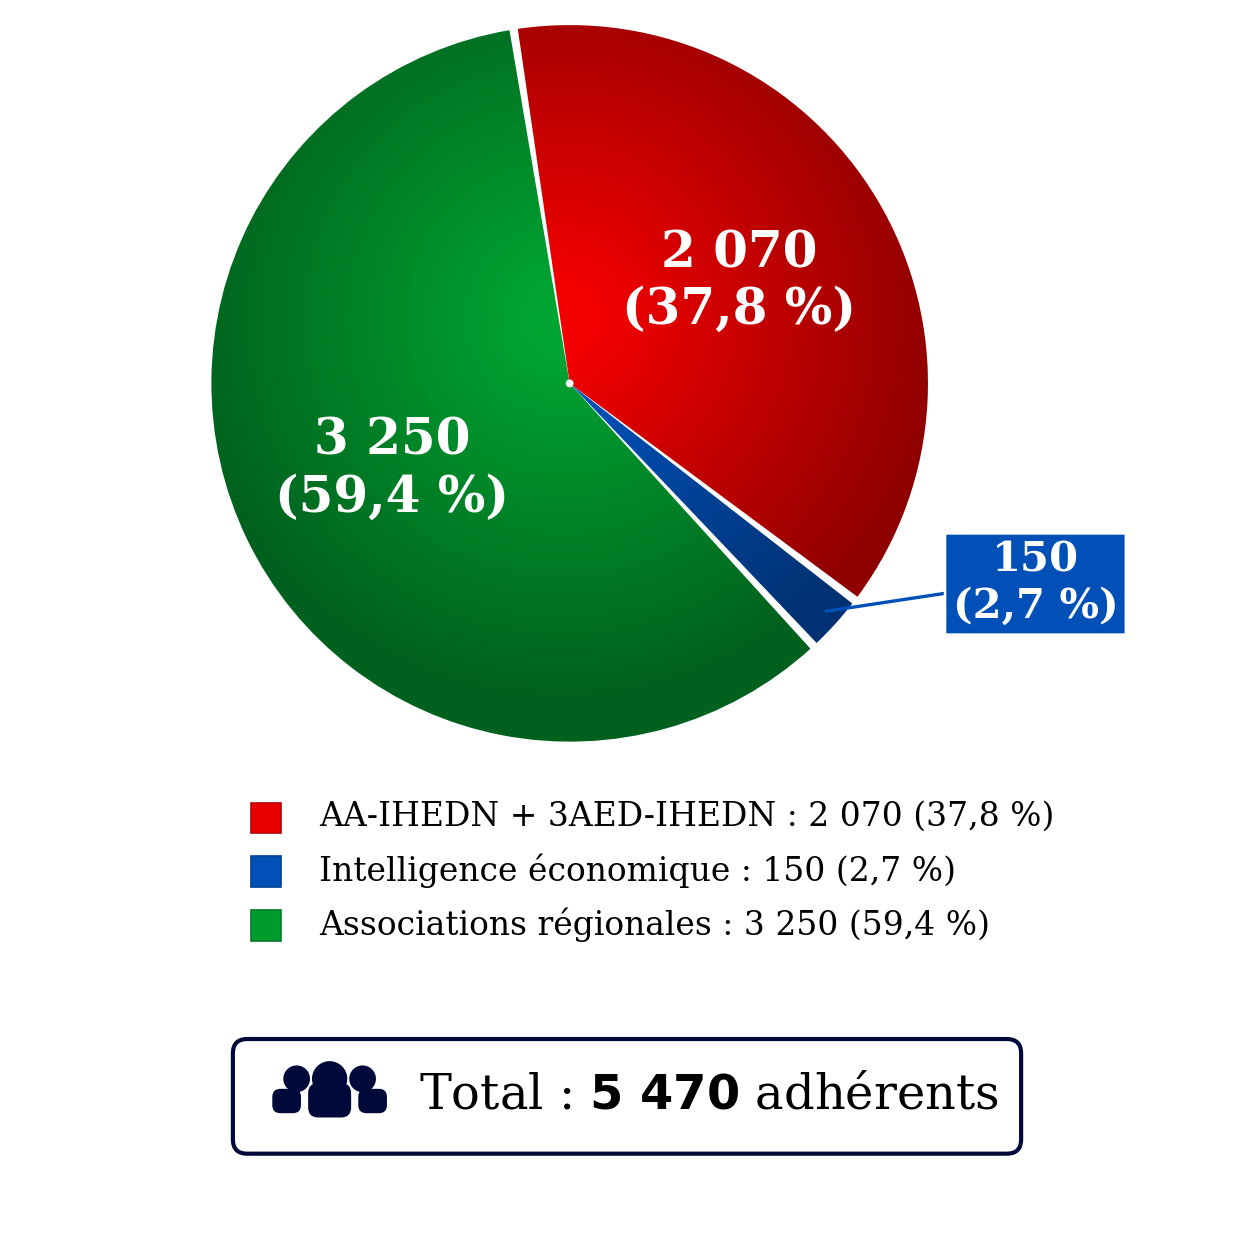
\includegraphics[width=\textwidth]{Figures/repartition_adherents_par_categorie}
        \caption{Répartition des adhérents par catégorie}
        \label{fig:repartition_adherents}
    \end{subfigure}
    \hfill
    \begin{subfigure}[b]{0.48\textwidth}
        \centering
        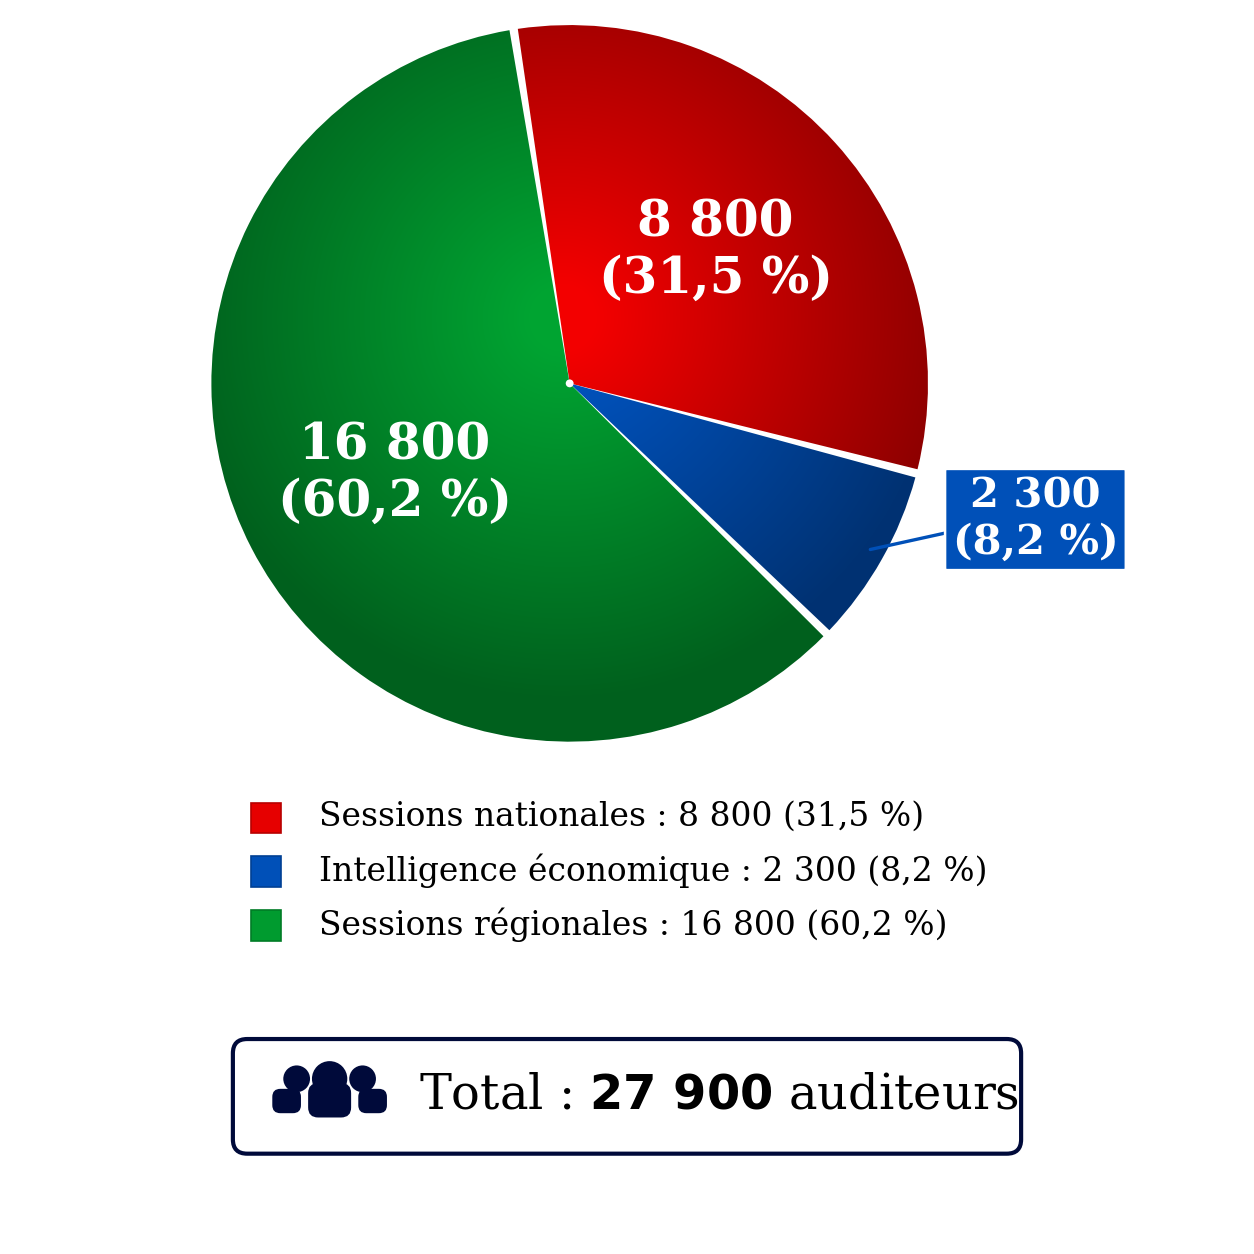
\includegraphics[width=\textwidth]{Figures/repartition_auditeurs_par_categorie}
        \caption{Répartition des auditeurs par catégorie}
        \label{fig:repartition_auditeurs}
    \end{subfigure}

    \caption{Comparaison de la répartition des adhérents et des auditeurs selon les différentes catégories de formation IHEDN.}
    \label{fig:comparaison_repartition_categories}
\end{figure}

Ces données mettent en évidence un premier constat structurant : le nombre d'adhérents effectivement engagés dans les associations des auditeurs demeure relativement limité au regard du volume total des auditeurs formés par l'IHEDN depuis l'origine.

Ce constat conduit à relativiser fortement l'idée d'un vivier immédiatement mobilisable de plusieurs dizaines de milliers de personnes.

Même parmi les sessions les plus récentes, une majorité d'auditeurs ne s'engage pas dans une \AssociationUnionIHEDN. Le taux d'adhésion observé ne doit donc pas être interprété comme un simple indicateur d'appartenance, mais comme un indice partiel du maintien d'un lien associatif après la session.

Par ailleurs, ces chiffres doivent être interprétés avec prudence. L'annuaire ne distingue pas les auditeurs décédés et agrège l'ensemble des promotions depuis les origines des sessions nationales et régionales. Le vivier théorique présenté par l'annuaire ne correspond donc pas nécessairement à une capacité réelle d'engagement.

Cette distinction entre potentiel théorique et potentiel effectivement mobilisable constitue un enjeu central de la réflexion.

L'annuaire fait également apparaître une érosion de l'adhésion avec l'ancienneté des sessions, phénomène qui peut tenir à l'âge, à l'évolution des disponibilités, aux trajectoires professionnelles ou encore à l'intensité variable du lien associatif.

Ce constat ne relève pas uniquement d'une donnée démographique. Il souligne l'intérêt de mieux comprendre les ressorts de l'adhésion, les causes de son érosion et les formes concrètes d'engagement dans les activités associatives.

\subsubsection{Évolution des taux d'adhésion selon les générations d'auditeurs}

Pour les sessions régionales, l'analyse des données fait apparaître une progression importante du taux d'adhésion parmi les promotions les plus récentes, comme en témoigne la figure \ref{fig:adhesion_sr}.

\begin{figure}[H]
    \centering
    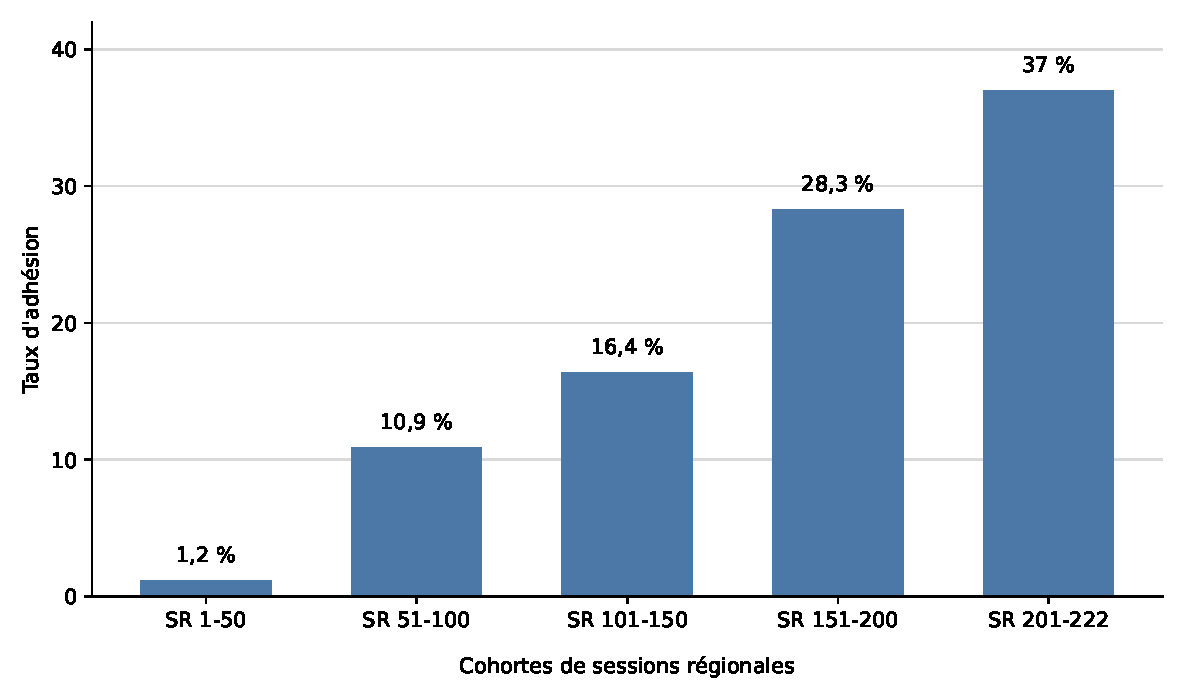
\includegraphics[width=0.8\linewidth]{Figures/graphe_adhesion_sr.pdf}
    \caption{Évolution du taux d'adhésion des auditeurs des sessions régionales selon les cohortes de sessions.}
    \label{fig:adhesion_sr}
\end{figure}
\vspace{-0.8\baselineskip}

Les sessions régionales les plus anciennes affichent des taux d'adhésion particulièrement faibles, tandis que les promotions plus récentes conservent généralement un lien plus étroit avec leur association régionale de rattachement. Cette diminution progressive du taux d'adhésion au fil du temps semble ainsi largement corrélée au vieillissement des auditeurs.

\newcounter{noteSessionRegionaleCentVingtTrois}
\newcounter{noteSessionRegionaleCentQuaranteTrois}
\newcounter{noteSessionRegionaleCentQuatreVingt}
\newcounter{noteSessionRegionaleDeuxCents}
\newcounter{noteSessionRegionaleDeuxCentDixNeuf}
\newcounter{noteSessionsRegionalesPublic}
À titre indicatif, les participants des sessions régionales 123 (1995)\footnotemark\setcounter{noteSessionRegionaleCentVingtTrois}{\value{footnote}}, 143 (2000)\footnotemark\setcounter{noteSessionRegionaleCentQuaranteTrois}{\value{footnote}}, 180 (2010)\footnotemark\setcounter{noteSessionRegionaleCentQuatreVingt}{\value{footnote}}, 200 (2015)\footnotemark\setcounter{noteSessionRegionaleDeuxCents}{\value{footnote}} et 219 (2020)\footnotemark\setcounter{noteSessionRegionaleDeuxCentDixNeuf}{\value{footnote}} étaient âgés de 30 à 55 ans au moment de leur formation\footnotemark\setcounter{noteSessionsRegionalesPublic}{\value{footnote}}.
\footnotetext[\value{noteSessionRegionaleCentVingtTrois}]{\cite{JORF:123_AR}.}
\footnotetext[\value{noteSessionRegionaleCentQuaranteTrois}]{\cite{JORF:143_AR}.}
\footnotetext[\value{noteSessionRegionaleCentQuatreVingt}]{\cite{JORF:180_AR}.}
\pagebreak[3]
%En 2025, les âges seraient donc de 60--85 ans (SR 123) et de 45--70 ans (SR 180).
En 2025, les auditeurs de la 123e session régionale auraient ainsi entre 60 et 85 ans, tandis que ceux de la 180e session régionale seraient âgés de 45 à 70 ans.
\footnotetext[\value{noteSessionRegionaleDeuxCents}]{\cite{JORF:200_AR}.}
\footnotetext[\value{noteSessionRegionaleDeuxCentDixNeuf}]{\cite{ihedn:219_AR}.}
\footnotetext[\value{noteSessionsRegionalesPublic}]{\cite{ihedn:description_AR}.}

Cette évolution démographique contribue vraisemblablement à expliquer l'érosion des effectifs des adhérents. Elle s'accompagne en effet de transformations des disponibilités personnelles et professionnelles, mais également d'un affaiblissement progressif des réseaux de sociabilité constitués à l'occasion des sessions, lesquels tendent naturellement à se distendre avec le temps.

L'analyse des sessions nationales, illustrée sur la figure \ref{fig:adhesion_sn}, met également en évidence des taux d'adhésion globalement plus élevés.

\begin{figure}[H]
    \centering
    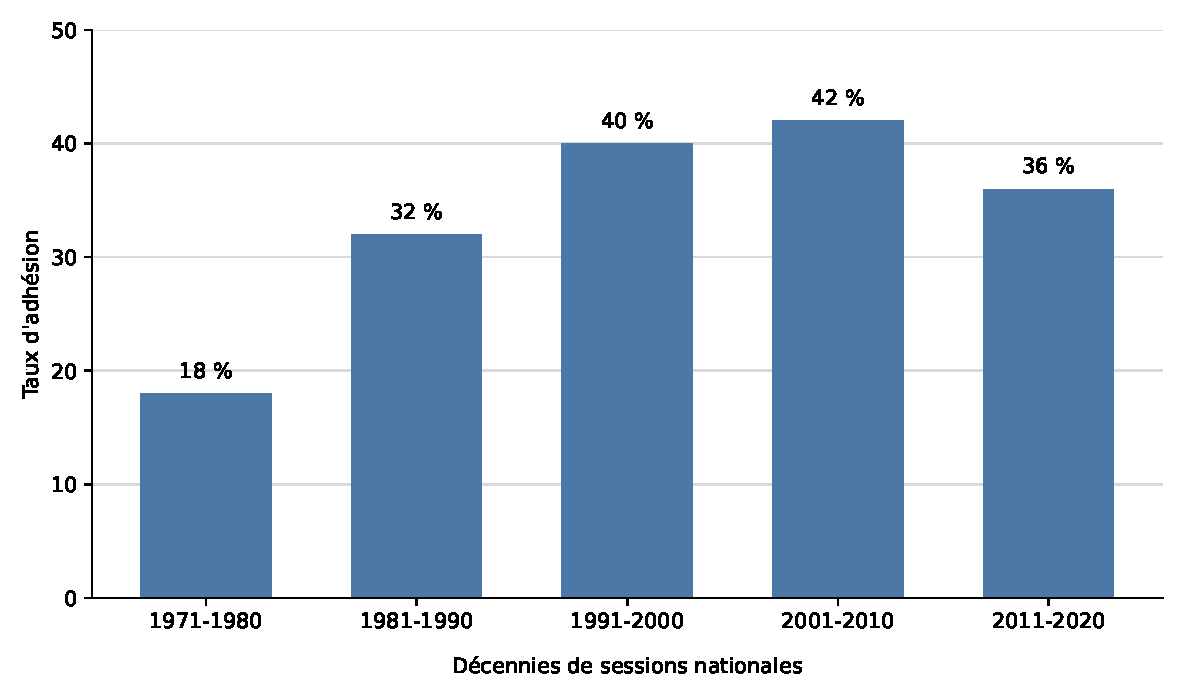
\includegraphics[width=0.85\linewidth]{Figures/graphe_adhesion_sn.pdf}
    \caption{Évolution du taux d'adhésion des auditeurs des sessions nationales selon les décennies.}
    \label{fig:adhesion_sn}
\end{figure}

Les auditeurs des sessions nationales apparaissent davantage enclins à adhérer à leur association dédiée. Cette situation peut notamment s'expliquer par la centralité institutionnelle des sessions nationales, des logiques de réseau professionnel plus fortes, une sociabilité plus durable ainsi que par le prestige associé à ces formations.

\subsubsection{Une structuration territoriale inégale des associations régionales}

Les données disponibles mettent également en évidence une forte hétérogénéité entre les associations régionales. Leurs effectifs sur le territoire métropolitain varient d'une vingtaine de membres pour l'AR~5 -- Bretagne occidentale à environ 380 membres pour l'\ARSeize{} -- Paris--Île-de-France.

Les associations régionales les plus importantes, c'est-à-dire comptant plus de 100 membres, sont notamment\footnote{La liste complète des \AssociationsRegionalesIHEDN{} ainsi que la localisation de leur siège sont présentées dans le tableau \ref{tab:associations_regionales_ihedn} en annexe \ref{annexe:maillage_territorial_ihedn}.} :
\begin{itemize}
    \item l'\ARSeize{} -- Paris--Île-de-France (380 membres) ;
    \item l'AR~14 -- Région lyonnaise (367 membres) ;
    \item l'AR~1 -- Aquitaine (environ 220 membres) ;
    \item l'AR~7 -- Centre-Val de Loire (environ 180 membres) ;
    \item les AR~2 -- Auvergne, 10 -- Franche-Comté, 15 -- Région Nord et 19 -- Occitanie Pyrénées (environ 140 membres) ;
    \item les AR~9 -- Provence et 12 -- Languedoc-Roussillon (environ 120 membres) ;
    \item les AR~6 -- Haute Bretagne, 8 -- Dauphiné-Savoie, 13 -- Lorraine, 18 -- Poitou-Charentes, 21 -- Versailles--Yvelines--Hauts-de-Seine, 22 -- Alsace et 29 -- Nice Côte d'Azur (environ 100 membres).
\end{itemize}

Les autres associations régionales comptent généralement moins de 60 membres.

La figure \ref{fig:carte_AR} présente la répartition territoriale des associations régionales en fonction de leurs effectifs approximatifs.

\begin{figure}[H]
\centering
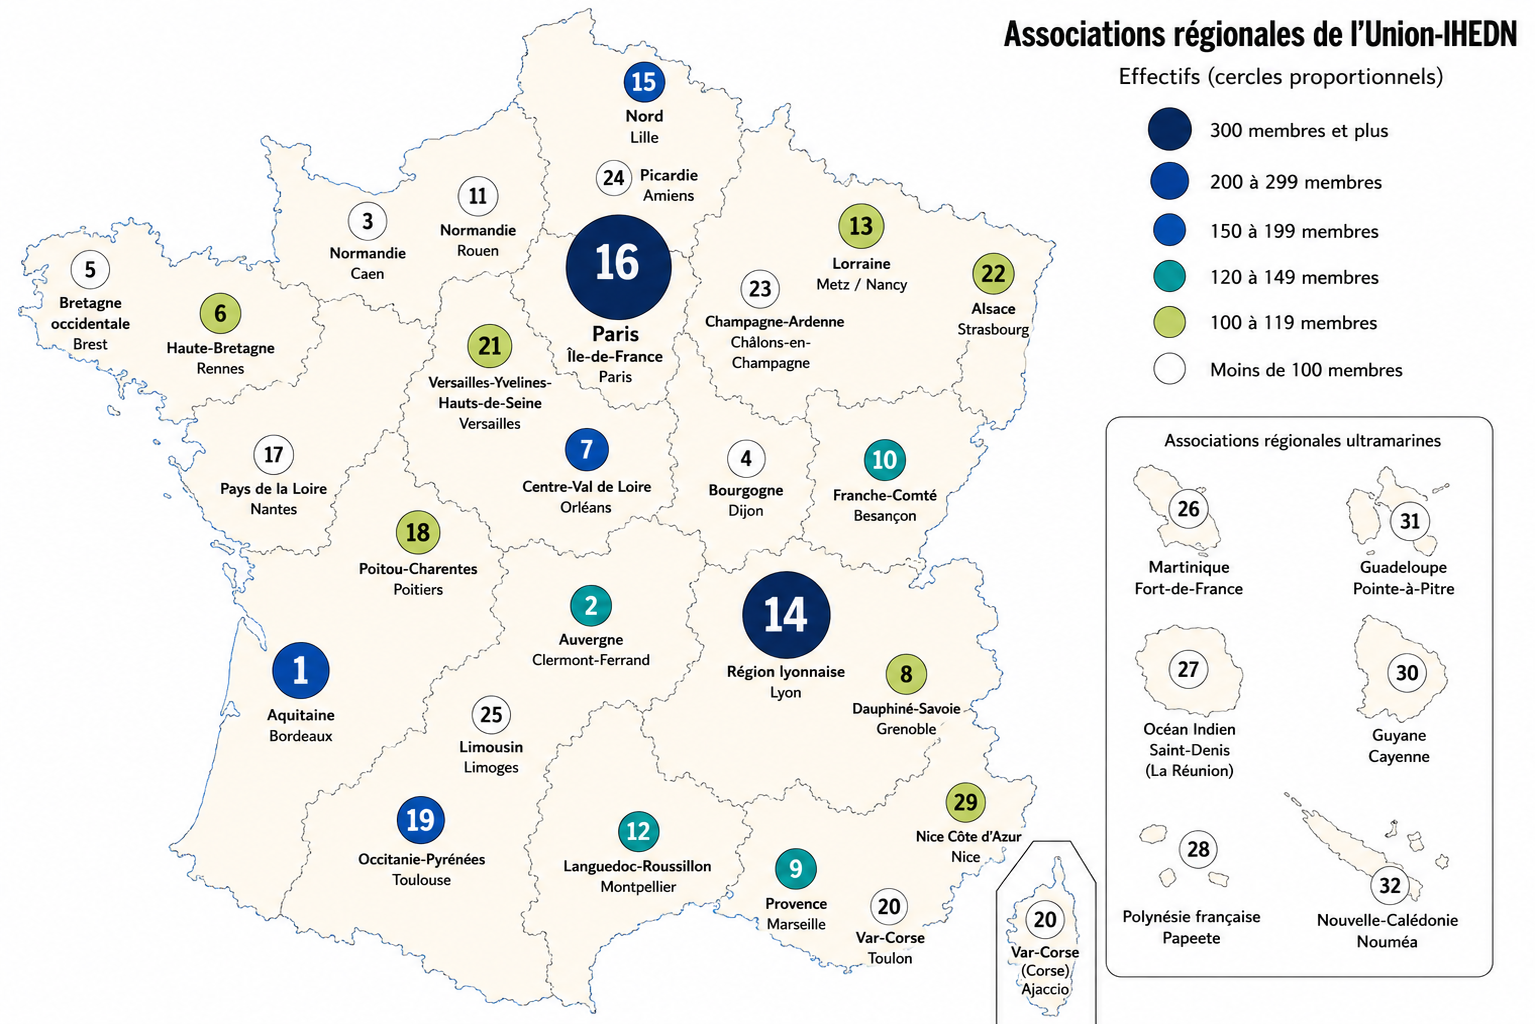
\includegraphics[width=\linewidth]{Figures/carte_AR}
\caption[Répartition territoriale des \AssociationsRegionalesIHEDN{} et importance relative de leurs effectifs.]{Répartition territoriale des \AssociationsRegionalesIHEDN{} et importance relative de leurs effectifs\footnotemark.}
\label{fig:carte_AR}
\end{figure}

\footnotetext{Chaque cercle porte le numéro de l'association régionale concernée, afin de faciliter son identification sur la carte.}

Cette dispersion des effectifs invite à distinguer le vivier national théorique, constitué par l'ensemble des quelque 28\,000 auditeurs, du vivier associatif réellement atteignable par une enquête administrée aux seuls adhérents.

Elle conduit également à poser explicitement la question du périmètre de l'étude : celui-ci pourrait être celui des personnes sensibilisées aux enjeux de défense, soit l'ensemble des auditeurs recensés. Toutefois, dans un premier temps, l'enquête envisagée vise principalement à objectiver les capacités réelles du périmètre associatif effectivement mobilisable.

L'annuaire ne renseigne pas sur l'activité effective des adhérents au sein des associations. Seule une enquête auprès des membres permettrait ainsi de mieux comprendre les ressorts de l'adhésion et de son érosion, mais également les conditions concrètes de l'engagement effectif dans les activités associatives.

Cette limite empêche de valoriser pleinement les capacités potentielles du réseau des auditeurs. La mise en place d'un outil dédié apparaît dès lors comme une étape préalable indispensable pour mieux connaître les profils, apprécier les disponibilités réelles et définir, le cas échéant, des formes d'implication adaptées aux différentes temporalités de la gestion de crise.

\subsection{Assurer une reconnaissance institutionnelle}

Toute relation utile avec les acteurs de la gestion de crise suppose une identification claire, un cadre d'action défini et une utilité reconnue par les autorités. Ces trois éléments constituent le socle de la démarche.

La cartographie proposée doit ainsi être comprise comme un levier de lisibilité institutionnelle. Elle ne vise pas seulement à recenser des profils, mais à rendre plus compréhensible, pour les autorités et les partenaires, la nature des compétences présentes au sein des associations.

Disposer d'éléments factuels permettra d'étayer les échanges avec préfets, maires et acteurs de la sécurité civile, d'examiner les conditions d'une articulation avec les dispositifs existants et d'explorer les appuis qui pourraient être apportés aux côtés des \glspl{dmd}\footcite{DMD_def_missions}.

\propositiongroup{Établir une cartographie de compétences}

Les propositions qui suivent déclinent cette orientation générale en six volets complémentaires, depuis la clarification institutionnelle jusqu'aux conditions de mise en \oe{}uvre et d'exploitation durable du dispositif.

\begin{subproposition}{Renforcer la lisibilité institutionnelle des \AssociationsUnionIHEDN}
Le comité considère que le questionnaire pourrait constituer un outil de structuration et de légitimation des compétences disponibles au sein des \AssociationsUnionIHEDN, afin de faciliter le dialogue avec les autorités publiques, d'améliorer la lisibilité du réseau associatif et d'examiner les conditions d'une articulation avec les dispositifs existants de gestion de crise.
\end{subproposition}

Cette reconnaissance institutionnelle ne peut toutefois reposer sur une affirmation générale du potentiel des auditeurs. Elle suppose de disposer d'éléments objectivés, construits selon une démarche suffisamment rigoureuse pour être exploitables et discutables.

\subsection{Une démarche d'objectivation}

Le comité propose de recourir à un questionnaire afin de disposer d'une connaissance plus fiable et plus exploitable des membres. Il ne s'agit ni d'une simple actualisation administrative, ni d'une opération de communication, mais d'un instrument destiné à mieux apprécier les ressources humaines, les expertises et les motivations susceptibles d'être mobilisées au sein des \AssociationsUnionIHEDN.

Cette réflexion s'inscrit dans la continuité de travaux antérieurs relatifs à la création d'une réserve, étudiée à la demande d'Édouard Philippe en 2015\footcite{DESAINTSALVY2026}. Elle trouve également un écho dans des analyses récentes émanant de personnalités de premier plan au sein de l'IHEDN. Anne-François de Saint Salvy (Vice-amiral d'escadre (2S) et Vice-président de l'Association des anciens auditeurs de l'IHEDN) souligne ainsi, dans son article « Comment mobiliser les auditeurs de l'IHEDN ? » paru en mars 2026\footcite{DESAINTSALVY2026} :

\begin{quote}
« Il est temps aujourd'hui de reprendre ce projet, sans doute d'une manière simplifiée et de se mettre en mesure de tirer profit des multiples compétences qu'apportent les auditeurs de l'IHEDN. Au-delà d'un statut et d'une organisation, le premier pas est sans doute celui d'un recensement des compétences disponibles, inscrites dans une grille permettant de les utiliser efficacement et tenu à jour régulièrement. »
\end{quote}

Cette démarche s'inscrit par ailleurs dans un contexte institutionnel marqué par un intérêt croissant pour la contribution des citoyens engagés et des réseaux associatifs à la préparation et à la gestion des crises majeures. La lettre adressée par l'IHEMI le 30 décembre 2025 relative aux enjeux liés aux risques et aux crises illustre cette dynamique\footcite{IHEMI:2025:LIREC75}. Elle souligne l'intérêt de mieux identifier et valoriser les ressources disponibles au sein des réseaux d'acteurs engagés afin de renforcer leur contribution aux actions de sensibilisation, de préparation, d'analyse et de retour d'expérience.

Dans cette perspective, le questionnaire proposé par le comité constitue un premier outil permettant de transformer cette ambition en une démarche concrète de connaissance et de structuration des ressources disponibles. Il vise à recueillir des données qualitatives et quantitatives utiles pour apprécier les formes possibles d'implication des membres des \AssociationsUnionIHEDN et à fournir une base objective pour orienter les réflexions futures de l'association.

Cette démarche pourrait s'inscrire dans le cadre du cinquantième anniversaire de l'\ARSeize{}. Cette échéance offre un cadre particulièrement propice pour engager une réflexion collective sur l'histoire de l'association, ses ressources et sa capacité d'adaptation face aux défis contemporains.

Le cheminement suivi par le comité confirme que le questionnaire ne constitue pas une proposition isolée, mais l'aboutissement d'une démarche progressive de cadrage, de recherche documentaire, de consultations méthodologiques et d'échanges institutionnels. Cette chronologie de travail, présentée en annexe \ref{annexe:cheminement_questionnaire}, permet de situer l'outil proposé dans la continuité des précédents identifiés et de préciser les conditions de crédibilité nécessaires à son éventuelle mise en \oe{}uvre.

\begin{subproposition}{Mettre en place un questionnaire de cartographie des compétences}
Le comité propose l'élaboration et la diffusion d'un questionnaire visant à identifier les compétences, les disponibilités et les capacités potentielles de contribution des adhérents des associations en matière de résilience et de gestion des crises majeures.
\end{subproposition}

Les données ainsi recueillies n'auront toutefois de portée que si elles peuvent être organisées, actualisées et exploitées dans un cadre structuré.

\subsection{Mise en \oe{}uvre d'une base de données de compétences}

Le questionnaire vise à cartographier les compétences, identifier les disponibilités et structurer une base de données exploitable. Les principaux objectifs opérationnels associés à cette démarche sont présentés dans le tableau \ref{tab:objectifs_questionnaire}.

\begin{table}[H]
\centering
\footnotesize
\setlength{\tabcolsep}{4pt}

\resizebox{\linewidth}{!}{%
\begin{tabular}{@{}>{\raggedright\arraybackslash}p{4cm}>{\raggedright\arraybackslash}p{7.5cm}>{\raggedright\arraybackslash}p{5.5cm}@{}}
\toprule

\textbf{Axe d'action} &
\textbf{Proposition} &
\textbf{Objectif} \\

\midrule

Cartographie des compétences &
Élaborer et diffuser un questionnaire auprès des adhérents des associations afin d'identifier leurs domaines d'expertise, leurs compétences, leurs disponibilités déclarées et leurs formes possibles de contribution. &
Disposer d'une vision consolidée et réaliste du potentiel associatif. \\

\addlinespace

Base de données centralisée &
Constituer une base de données regroupant les compétences identifiées, exploitable par les associations dans un cadre conforme aux règles de protection des données. &
Faciliter la préparation, l'analyse et le dialogue institutionnel, sans présumer d'une mobilisation opérationnelle. \\

\addlinespace

Hypothèse de dispositif d'appui &
Étudier, à partir des données recueillies, les conditions et les limites d'un éventuel dispositif d'appui associatif, en lien avec les instances de l'IHEDN et les autorités compétentes. &
Apprécier les formes de contribution envisageables sans créer de chaîne autonome de gestion de crise. \\

\addlinespace

Analyse du dispositif antérieur &
Analyser les raisons ayant conduit à l'interruption de la précédente réserve des auditeurs. &
Tirer les enseignements nécessaires avant toute réactivation. \\

\addlinespace

Identification des formes d'engagement &
Identifier les membres volontaires, les domaines dans lesquels ils accepteraient de contribuer et les contraintes qui encadrent cette disponibilité. &
Assurer la crédibilité du dispositif et éviter toute surestimation des capacités réelles. \\

\bottomrule
\end{tabular}
}

\caption[Objectifs structurants du questionnaire]{Objectifs structurants associés à la mise en place du questionnaire de cartographie des compétences du réseau associatif IHEDN.}
\label{tab:objectifs_questionnaire}

\end{table}

\begin{subproposition}{Structurer une base de données des compétences mobilisables}
Les informations recueillies pourraient permettre la constitution d'une base de données des compétences, destinée à mieux identifier les ressources disponibles dans le cadre d'actions de préparation, d'analyse ou de retour d'expérience.
\end{subproposition}

Dans la perspective de concevoir ce questionnaire, le comité a fait appel à l'expertise du docteur Victor Violier, sociologue à l'\gls{irsem}\footcite{violier_irsem}, afin de disposer de fondements méthodologiques solides et d'en encadrer la mise en \oe{}uvre\footnote{Entretien avec le docteur Victor Violier, sociologue à l'\gls{irsem}, réalisé le 20 février 2026.}.

\subsection{Cadre méthodologique}

Sur la base des conseils du docteur Violier, la démarche doit s'inscrire dans une logique sociologique d'objectivation des données, afin de dépasser les représentations spontanées\footnote{\textit{Ibid.}}.

Les données issues de l'annuaire 2022 invitent à préciser le périmètre de l'enquête. Si le questionnaire est adressé aux seuls adhérents, il mesurera d'abord la capacité d'engagement des \AssociationsUnionIHEDN. S'il devait être étendu à un cercle plus large d'auditeurs, il poserait d'autres difficultés : accès aux coordonnées, actualisation des fichiers, statut des personnes inactives ou décédées, conformité juridique et interprétation des non-réponses. Le comité retient donc une approche progressive, centrée sur un périmètre maîtrisable, tout en signalant explicitement les limites de représentativité qui en découlent.

La construction du questionnaire devra respecter plusieurs principes méthodologiques. Il conviendra d'abord d'éviter toute imposition de problématique\footcite{Bourdieu1986}, en formulant des questions neutres et non orientées, afin de ne pas influencer les réponses et de préserver la fiabilité des données recueillies. Il faudra également tenir compte du risque d'« illusion biographique », entendue, au sens de Pierre Bourdieu, comme la tendance des individus à reconstruire \textit{a posteriori} leur trajectoire de manière cohérente et linéaire\footcite[69]{Bourdieu1986}. Dans le cadre du questionnaire, ce biais peut conduire les répondants à surestimer la cohérence de leur parcours ou à présenter leurs compétences de manière rétrospectivement rationalisée, au détriment d'une description plus nuancée de leurs expériences et de leurs capacités réelles. Enfin, une attention particulière devra être portée à l'équilibre entre questions ouvertes et questions fermées\footcite[65]{Fenneteau2015}.

Sur le plan juridique, la démarche devra être conforme au \gls{rgpd}\footcite{RGPD_CNIL}, ainsi qu'aux exigences en matière de protection des données et aux principes d'anonymisation.

\begin{subproposition}{Garantir un encadrement méthodologique et juridique du questionnaire}
Le comité considère que la conception du questionnaire doit reposer sur une méthodologie rigoureuse, fondée sur des principes d'objectivation des données, de neutralité des questions et de clarification du périmètre enquêté, tout en garantissant la conformité du dispositif au \gls{rgpd} et aux exigences de protection des données personnelles.
\end{subproposition}

La mise en place de ce questionnaire permettrait à l'association de disposer d'éléments plus concrets pour préciser son rôle, documenter ses compétences internes et, le cas échéant, présenter une contribution lisible aux différents niveaux des associations et de l'IHEDN. La question de sa diffusion vers les autorités publiques et de sa reconnaissance institutionnelle constitue dès lors le prolongement de cette démarche.


\section{Plan prévisionnel de mise en \oe{}uvre du questionnaire}

Le plan d'action proposé détaille les modalités de conception, de déploiement et d'exploitation de ce questionnaire, dans une logique de gestion de projet étendue jusqu'à septembre 2027.

\subsection{Planification et structuration des tâches}

La réalisation du questionnaire s'inscrit dans une démarche progressive, structurée autour de plusieurs phases complémentaires :

\begin{enumerate}
    \item \textbf{Phase de cadrage stratégique}
    \begin{itemize}
        \item Réalisation d'une étude bibliographique approfondie (octobre 2025 - avril 2026) permettant de consolider le cadre conceptuel et méthodologique ;
        \item Obtention d'une validation institutionnelle formelle (\UnionIHEDN, Bureau, \acrshort{codir}), condition préalable à tout déploiement ;
        \item Sélection de trois \AssociationsRegionalesIHEDN{} pilotes afin de tester et valider le dispositif.
    \end{itemize}

    \item \textbf{Phase de conception du questionnaire}
    \begin{itemize}
        \item Définition de l'objectif général, des thématiques et de la problématique centrale ;
        \item Élaboration d'une trame structurée et d'une grille d'exploitation des données ;
        \item Conception du contenu détaillé et d'une maquette du questionnaire\footnote{cf. annexe \ref{annexe:maquette_questionnaire}} ;
        \item Choix des outils techniques et du support de diffusion.
    \end{itemize}

    \item \textbf{Phase d'identification des ressources}
    \begin{itemize}
        \item Identification des compétences nécessaires (experts en sciences sociales, spécialistes RGPD, partenaires académiques) ;
        \item Structuration des partenariats (\UnionIHEDN, \gls{irsem}, institutions académiques) ;
        \item Estimation des ressources et planification détaillée.
    \end{itemize}

    \item \textbf{Phase de lancement et de déploiement}
    \begin{itemize}
        \item Mise en place d'un comité de pilotage ;
        \item Communication interne et externe sur les objectifs du projet ;
        \item Préparation et diffusion de la campagne par l'intermédiaire de courriers électroniques ;
        \item Administration du questionnaire auprès des membres.
    \end{itemize}

    \item \textbf{Phase d'exploitation et de valorisation}
    \begin{itemize}
        \item Traitement et analyse des données collectées ;
        \item Production d'indicateurs et de cartographies de compétences ;
        \item Rédaction d'un rapport de travail et capitalisation des résultats ;
        \item Restitution finale prévue le 15 septembre 2027.
    \end{itemize}
\end{enumerate}

Cette organisation suit un cycle complet de projet, de la conception à la valorisation, en cohérence avec l'objectif du comité : renforcer la capacité d'analyse de l'Union-IHEDN et rendre plus lisible la contribution possible de ses associations face aux crises majeures.

\subsection{Organisation proposée des acteurs : une gouvernance en triptyque}

Un tel projet nécessite des responsabilités clairement identifiées, afin de garantir un suivi méthodologique rigoureux.

Pour cela, une gouvernance en triptyque est proposée. Celle-ci se composerait d'abord d'un comité de pilotage, chargé d'assurer l'orientation stratégique, la validation des grandes étapes et le lien avec les instances décisionnelles. Un comité scientifique apporterait ensuite une validation méthodologique et contribuerait à la conformité juridique du dispositif. Enfin, la conception et la mise en \oe{}uvre seraient assurées par une équipe projet composée de membres du comité.

Une telle gouvernance, illustrée dans la figure \ref{fig:gouvernance-triptyque}, permettrait d'articuler expertise, légitimité institutionnelle et capacité de suivi, trois conditions nécessaires à la réussite d'une enquête de cette ampleur.

\begin{figure}[H]
\centering
\scalebox{0.8}{%
\begin{tikzpicture}[
    governance circle/.style={draw=black, line width=1.1pt, fill=gray!3},
    governance title/.style={font=\bfseries\footnotesize, align=center, text width=3.8cm},
    governance body/.style={font=\scriptsize, align=center, text width=3.6cm, anchor=north, inner sep=0pt},
    interaction arrow/.style={-{Stealth[length=2.4mm]}, line width=0.65pt},
    interaction label/.style={font=\tiny, align=center, fill=white, inner sep=1.2pt}
]
\def\governanceradius{2.05}
\coordinate (pilotage) at (0,2.15);
\coordinate (scientifique) at (-3.15,-1.25);
\coordinate (projet) at (3.15,-1.25);

\draw[governance circle] (pilotage) circle[radius=\governanceradius cm];
\draw[governance circle] (scientifique) circle[radius=\governanceradius cm];
\draw[governance circle] (projet) circle[radius=\governanceradius cm];

\draw[interaction arrow] (0.72,0.40) to[bend left=12]
    node[interaction label, pos=0.50, sloped, above] {Orientation\\Validation} (1.52,-0.05);
\draw[interaction arrow] (1.06,0.05) to[bend left=12]
    node[interaction label, pos=0.50, sloped, below] {Reporting} (0.26,0.50);

\draw[interaction arrow] (-0.72,0.40) to[bend right=12]
    node[interaction label, pos=0.50, sloped, above] {Cadrage\\Arbitrage} (-1.52,-0.05);
\draw[interaction arrow] (-1.06,0.05) to[bend right=12]
    node[interaction label, pos=0.50, sloped, below] {Avis\\Conformité} (-0.26,0.50);

\draw[interaction arrow] (-1.25,-1.05) to[bend left=10]
    node[interaction label, pos=0.50, above] {Appui méthodologique\\et RGPD} (1.25,-1.05);
\draw[interaction arrow] (1.25,-1.45) to[bend left=10]
    node[interaction label, pos=0.50, below] {Besoins terrain\\Retours opérationnels} (-1.25,-1.45);

\node[governance title] at (0,2.80) {Comité de pilotage};
\node[governance body] at (0,2.42) {%
    Présidents des trois\\régions pilotes\\[0.08cm]
    Présidence de l'Union IHEDN\\[0.08cm]
    Membres du comité d'étude
};

\node[governance title] at (-3.15,-0.60) {Comité scientifique};
\node[governance body] at (-3.15,-0.98) {%
    Expert en études\\et enquêtes sociologiques\\[0.08cm]
    Juriste RGPD
};

\node[governance title] at (3.15,-0.60) {Équipe projet};
\node[governance body] at (3.15,-0.98) {%
    Membres opérationnels\\du comité
};
\end{tikzpicture}
}
\caption{Organisation proposée de la gouvernance du projet de questionnaire.}
\label{fig:gouvernance-triptyque}
\end{figure}

Le comité a également identifié les principaux risques susceptibles d'affecter l'aboutissement du projet.

\subsection{Analyse des risques et facteurs de vigilance}

Le tableau \ref{tab:risques} présente les risques identifiés, en cohérence avec les retours d'expérience issus des travaux du comité.

\begin{table}[h]
\centering
\setlength{\tabcolsep}{4pt}
\makebox[\linewidth][c]{%
\begin{tabular}{@{}>{\raggedright\arraybackslash}p{3cm}>{\raggedright\arraybackslash}p{8.8cm}C{2.35cm}C{1.95cm}@{}}
\toprule
\textbf{Risque} & \textbf{Description} & \textbf{Probabilité} & \textbf{Impact} \\
\midrule
Coordination & Difficulté de coordination entre les trois \AssociationsRegionalesIHEDN{} pilotes & Moyenne & Élevé \\
\addlinespace
Interprétation & Mauvaise lecture ou instrumentalisation des résultats, pouvant générer inertie ou incompréhension & Faible & Élevé \\
\addlinespace
Participation & Retards ou faibles taux de réponse, compromettant la représentativité des données & Moyenne & Élevé \\
\addlinespace
Périmètre & Confusion possible entre le potentiel des adhérents répondants, celui des associations et celui de l'ensemble des auditeurs recensés & Moyenne & Élevé \\
\addlinespace
Ressources & Inadéquation potentielle entre les compétences requises pour assurer la qualité de conception et l'appropriation du questionnaire, et les ressources effectivement mobilisées & Faible & Élevé \\
\bottomrule
\end{tabular}
}
\caption{Cartographie des risques du projet.}
\label{tab:risques}
\end{table}

À ces risques s'ajoutent des points de vigilance déjà identifiés par le comité, notamment la disponibilité réelle des membres, la nécessité d'un socle commun de compétences, l'hétérogénéité des effectifs entre \AssociationsRegionalesIHEDN{} et l'importance d'une communication claire et pédagogique.

\begin{subproposition}{Mettre en œuvre une démarche progressive et encadrée}
Le comité considère que la mise en place du questionnaire doit s'inscrire dans une démarche progressive, fondée sur une coordination étroite entre les associations pilotes, une communication claire auprès des membres et une vigilance particulière quant à la qualité méthodologique et à l'interprétation des résultats.
\end{subproposition}

\subsection{Facteurs clefs de succès}

Les travaux du comité conduisent à identifier plusieurs conditions nécessaires à la réussite du projet. Celui-ci suppose d'abord une validation institutionnelle claire et un portage durable par les instances associatives concernées. Il repose également sur une conception méthodologique suffisamment rigoureuse pour garantir la crédibilité et l'exploitabilité des résultats recueillis.

L'adhésion des membres constitue un second enjeu majeur. Elle dépendra en partie de la capacité de l'association à expliquer les finalités du questionnaire, les modalités d'utilisation des données collectées et les bénéfices attendus pour les auditeurs comme pour les \AssociationsUnionIHEDN. L'analyse de l'annuaire 2022 rappelle que l'adhésion associative ne va pas de soi, y compris parmi les sessions récentes. La formulation du questionnaire devra donc permettre de comprendre les conditions concrètes de l'engagement, et non seulement de recueillir une disponibilité de principe.

Enfin, l'intérêt du dispositif reposera sur la capacité à produire une exploitation concrète des résultats, permettant de mieux identifier les compétences disponibles et de renforcer la lisibilité de l'\ARSeize{} auprès des autorités et partenaires institutionnels.

\begin{subproposition}{Inscrire le questionnaire dans une démarche durable et exploitable}
Le comité considère que la réussite du questionnaire dépendra autant de sa crédibilité méthodologique que de sa capacité à produire des résultats concrètement exploitables pour les \AssociationsUnionIHEDN{} et leurs partenaires institutionnels.
\end{subproposition}

Sur la base des éléments précédents, le comité a également étudié un calendrier prévisionnel, décrit dans la figure \ref{fig:gantt-questionnaire-ar16} en annexe \ref{annexe:figures_complementaires:calendrier_questionnaire} en vue d'engager une telle démarche.


\section{Conclusion}

Les travaux du comité mettent en évidence une réalité centrale : \textbf{les \AssociationsRegionalesIHEDN{} disposent probablement d'un potentiel significatif de contribution à la résilience nationale, mais celui-ci demeure aujourd'hui insuffisamment identifié}.

La spécificité des auditeurs réside dans la diversité de leurs parcours, leur culture stratégique commune et leur capacité à produire des analyses transversales. Cette valeur ajoutée ne relève pas d'une substitution aux autorités publiques, ni d'une gestion directe des crises par l'association.

Dans ce contexte, les \AssociationsRegionalesIHEDN{} peuvent agir principalement avant la crise, par la préparation, la sensibilisation et la mise en relation des compétences, puis après la crise, par l'analyse, la production de bilans de retour d'expérience et la diffusion des enseignements. Pendant l'événement, leur rôle collectif demeure nécessairement limité par les cadres juridiques, hiérarchiques et opérationnels existants.

La mise en place d'un questionnaire constitue, à cet égard, une étape déterminante. L'analyse de l'annuaire 2022 montre en effet que le nombre d'auditeurs recensés, le nombre d'adhérents et l'engagement effectif ne se recouvrent pas. Elle confirme que les associations ne peuvent fonder leur positionnement sur une simple estimation de vivier : elles doivent disposer de données actualisées, qualifiées et interprétées avec prudence.

Le questionnaire permettrait ainsi de passer d'une intuition générale sur la richesse du réseau à une connaissance objectivée des profils, des disponibilités, des domaines d'expertise et de la motivation à contribuer. Son intérêt n'est pas de présumer une mobilisation opérationnelle, mais de clarifier ce que les \AssociationsRegionalesIHEDN{} peuvent réellement apporter, dans quelles temporalités et sous quelles conditions institutionnelles.

Plus largement, ce travail ouvre une réflexion sur la place des citoyens engagés face aux crises contemporaines. Dans un contexte marqué par l'incertitude, une hybridation des menaces et des vulnérabilités informationnelles, la résilience nationale repose de plus en plus sur une orchestration institutionnelle, territoriale et sociétale.

Les \AssociationsRegionalesIHEDN{}, par leur nature et par leur réseau, peuvent y contribuer de manière crédible, en valorisant les compétences de leurs auditeurs, en renforçant la culture de résilience et en mettant leur capacité d'analyse, de préparation et de capitalisation au service de l'intérêt général.

\clearpage

\addtocontents{toc}{\protect\newpage}
\appendix
\section{Figures complémentaires}
\label{annexe:figures_complementaires}

\subsection{Quatre cercles structurant l'action de l'IHEDN}
\label{annexe:figures_complementaires:cercles_structurants_action_IHEDN}

\begin{figure}[H]
\centering
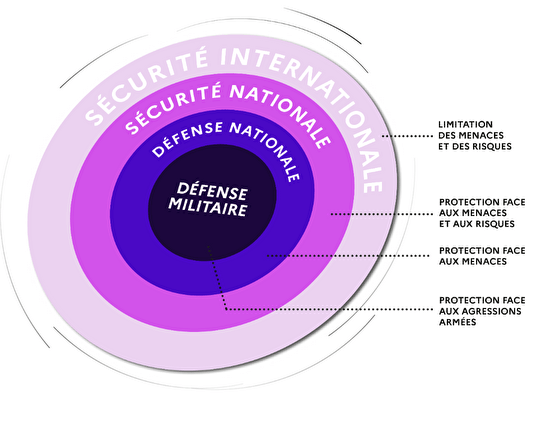
\includegraphics[width=0.8\linewidth]{Figures/cercles.png}
\caption[Quatre cercles structurant l'action de l'IHEDN]{Quatre cercles structurant l'action de l'IHEDN\footnotemark.}
\label{fig:cercles}
\end{figure}
\footnotetext{Illustration issue de : \cite{IHEDN_perimetre_defense_nationale}.}

\clearpage

\subsection{Chaîne opérationnelle de gestion de crise.}
\label{annexe:figures_complementaires:chaine_operationnelle_gestion_de_crise}

\begin{figure}[H]
\centering
\rotatebox{90}{%
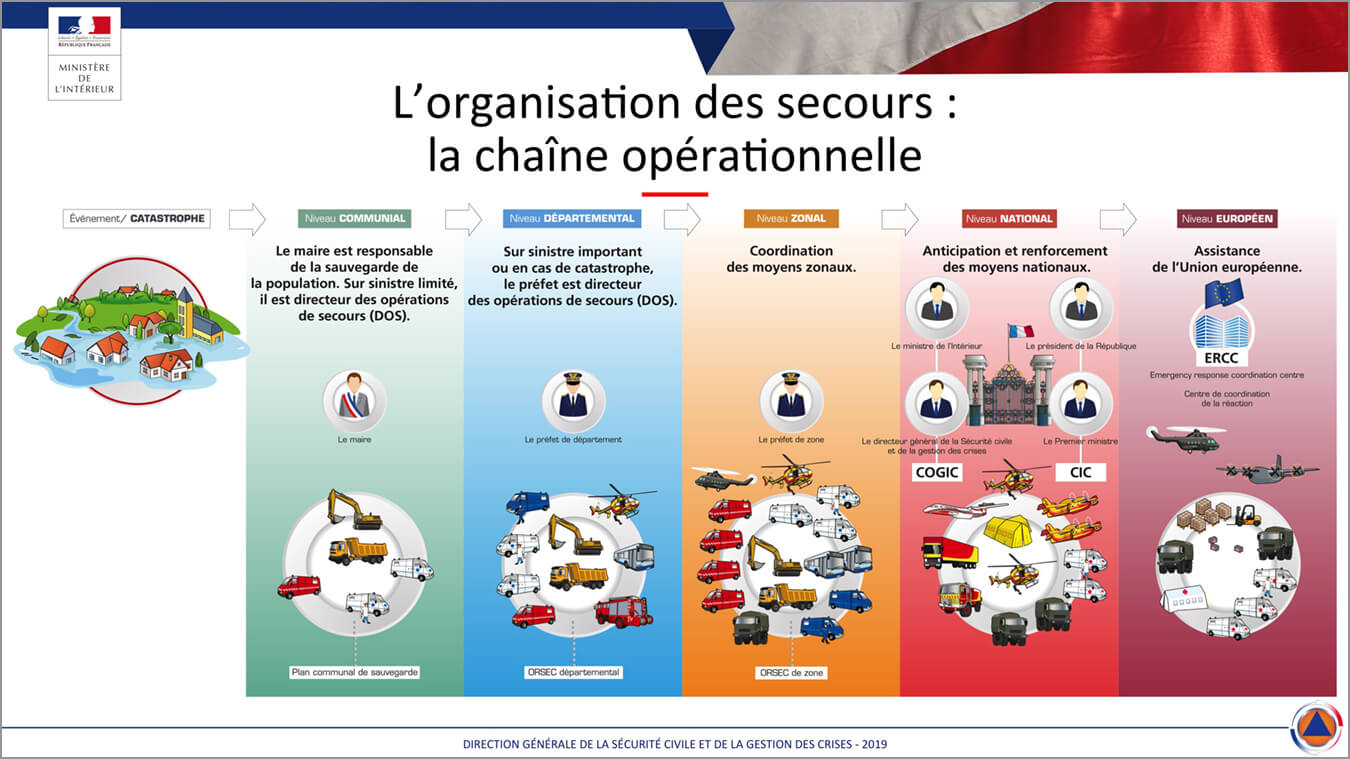
\includegraphics[width=0.82\textheight]{Figures/Chaine_operationnelle_gestion_crises.jpg}%
}
\caption[Chaîne opérationnelle de gestion de crise.]{Chaîne opérationnelle de gestion de crise\footnotemark.}
\label{fig:chaine_operationnelle}
\end{figure}

\footnotetext{Illustration issue de : \cite{dispositif_gestion_de_crise}.}

\clearpage

\subsection{Calendrier prévisionnel de mise en \oe{}uvre du questionnaire}
\label{annexe:figures_complementaires:calendrier_questionnaire}

La figure \ref{fig:gantt-questionnaire-ar16} présente l'enchaînement des différentes étapes du projet de mise en \oe{}uvre du questionnaire, depuis leur planification jusqu'à l'obtention et l'exploitation des résultats en septembre 2027.

\begin{figure}[H]
\centering
\makeatletter
\providecommand{\ganttvrulelabel}[4][]{%
  \begingroup
  \ganttset{#1}%
  \gtt@tsstojulian{#4}{\gtt@vrule@slot}%
  \gtt@juliantotimeslot{\gtt@vrule@slot}{\gtt@vrule@slot}%
  \pgfmathsetmacro\y@upper{%
    \gtt@lasttitleline * \ganttvalueof{y unit title}%
  }%
  \pgfmathsetmacro\y@lower{%
    \gtt@lasttitleline * \ganttvalueof{y unit title}%
    + (\gtt@currentline - \gtt@lasttitleline - 1)%
    * \ganttvalueof{y unit chart}%
  }%
  \pgfmathsetmacro\x@mid{%
    (\gtt@vrule@slot - 1 + \ganttvalueof{vrule offset})%
    * \ganttvalueof{x unit}%
  }%
  \pgfmathsetmacro\y@label{\y@lower - #2}%
  \draw [/pgfgantt/vrule]
    (\x@mid pt, \y@upper pt) -- (\x@mid pt, \y@label pt)
    node [/pgfgantt/vrule label node] {#3};%
  \endgroup
}
\makeatother

\begin{ganttchart}[
    hgrid,
    x unit=0.0147cm,
    y unit chart=0.58cm,
    time slot format=isodate,
    title/.style={fill=gray!20, draw=gray!60},
    title label font=\bfseries\fontsize{6.4pt}{7pt}\selectfont,
    bar label font=\fontsize{6.8pt}{7.4pt}\selectfont,
    group label font=\bfseries\fontsize{6.8pt}{7.4pt}\selectfont,
    bar height=0.60,
    group height=0.38,
    group right shift=0,
    group left shift=0,
    group peaks tip position=0,
    group peaks height=0.18,
    group peaks width=0.2,
    bar/.style={fill=gray!35, draw=gray!70},
    group/.style={fill=gray!70, draw=gray!80},
    vrule/.style={dashed, line width=0.6pt, draw=black!70},
    vrule offset=.5,
    vrule label font=\fontsize{5pt}{5.6pt}\selectfont,
    vrule label node/.append style={anchor=north, rotate=45, align=left, inner sep=0.5pt, text=black!80},
    canvas/.style={draw=gray!50},
    y unit title=0.58cm,
    title height=1,
    title label anchor/.style={below=-1.6ex},
    bar label node/.append style={text width=4.2cm, align=right},
    group label node/.append style={text width=4.2cm, align=right}
]{2025-10-01}{2027-09-30}

\gantttitle{2025}{92}
\gantttitle{2026}{365}
\gantttitle{2027}{273} \\
\gantttitle{Oct}{31}
\gantttitle{Nov}{30}
\gantttitle{Déc}{31}
\gantttitle{Jan}{31}
\gantttitle{Fév}{28}
\gantttitle{Mar}{31}
\gantttitle{Avr}{30}
\gantttitle{Mai}{31}
\gantttitle{Juin}{30}
\gantttitle{Juil}{31}
\gantttitle{Août}{31}
\gantttitle{Sep}{30}
\gantttitle{Oct}{31}
\gantttitle{Nov}{30}
\gantttitle{Déc}{31}
\gantttitle{Jan}{31}
\gantttitle{Fév}{28}
\gantttitle{Mar}{31}
\gantttitle{Avr}{30}
\gantttitle{Mai}{31}
\gantttitle{Juin}{30}
\gantttitle{Juil}{31}
\gantttitle{Août}{31}
\gantttitle{Sep}{30} \\

\ganttgroup{Cadrage stratégique}{2025-10-01}{2026-06-25} \\
\ganttbar[bar/.append style={fill=blue!35}]{Étude bibliographique}{2025-10-01}{2026-04-30} \\
\ganttbar[bar/.append style={fill=blue!25}]{Sélection des trois AR pilotes}{2026-04-01}{2026-05-31} \\
\ganttbar[bar/.append style={fill=blue!45}]{Validation institutionnelle}{2026-03-30}{2026-05-25} \\

\ganttgroup{Conception du questionnaire}{2026-02-01}{2026-12-31} \\
\ganttbar[bar/.append style={fill=green!35}]{Objectifs, problématique et thèmes}{2026-02-01}{2026-12-31} \\
\ganttbar[bar/.append style={fill=green!25}]{Trame et grille d'exploitation}{2026-06-01}{2026-12-31} \\
\ganttbar[bar/.append style={fill=green!45}]{Maquette, support et outils}{2026-06-01}{2026-08-31} \\

\ganttgroup{Mobilisation et gouvernance}{2026-07-01}{2026-12-31} \\
\ganttbar[bar/.append style={fill=orange!35}]{Comité de pilotage}{2026-07-01}{2026-09-30} \\
\ganttbar[bar/.append style={fill=orange!25}]{Comité scientifique}{2026-07-01}{2026-09-30} \\
\ganttbar[bar/.append style={fill=orange!45}]{Ressources et partenariats}{2026-07-01}{2026-09-30} \\
\ganttbar[bar/.append style={fill=green!55}]{Validation RGPD et consentement}{2026-10-01}{2026-12-31} \\
\ganttbar[bar/.append style={fill=orange!55}]{Communication projet}{2026-10-01}{2026-12-31} \\
\ganttbar[bar/.append style={fill=orange!65}]{Préparation de l'emailing}{2026-10-01}{2026-12-31} \\

\ganttgroup{Lancement et déploiement}{2027-01-04}{2027-03-31} \\
\ganttbar[bar/.append style={fill=red!30}]{Lancement du questionnaire}{2027-01-04}{2027-02-28} \\
\ganttbar[bar/.append style={fill=red!40}]{Administration et relances}{2027-02-28}{2027-03-31} \\

\ganttgroup{Exploitation et valorisation}{2027-04-01}{2027-09-15} \\
\ganttbar[bar/.append style={fill=purple!25}]{Traitement des résultats}{2027-04-01}{2027-05-31} \\
\ganttbar[bar/.append style={fill=purple!35}]{Analyse et cartographie des compétences}{2027-04-01}{2027-06-30} \\
\ganttbar[bar/.append style={fill=purple!45}]{Rédaction du rapport de travail}{2027-06-01}{2027-08-31} \\
\ganttbar[bar/.append style={fill=purple!55}]{Capitalisation et restitution}{2027-08-01}{2027-09-15}

\ganttvrulelabel[vrule/.append style={draw=blue!70!black}, vrule label node/.append style={anchor=north east}]{10}{\shortstack[l]{15/05/2026\\Validation CODIR / Bureau}}{2026-05-15}
\ganttvrulelabel[vrule/.append style={draw=blue!70!black}, vrule label node/.append style={anchor=north west}]{34}{\shortstack[l]{25/06/2026\\Restitution du rapport de comité}}{2026-06-25}
\ganttvrulelabel[vrule/.append style={draw=red!70!black}, vrule label node/.append style={anchor=north west}]{34}{\shortstack[l]{31/03/2027\\Clôture de l'enquête}}{2027-03-31}
\ganttvrulelabel[vrule/.append style={draw=purple!70!black}, vrule label node/.append style={anchor=north east}]{10}{\shortstack[l]{15/09/2027\\Restitution finale}}{2027-09-15}

\end{ganttchart}

\caption{Calendrier prévisionnel de mise en \oe{}uvre du questionnaire de cartographie des compétences des membres de l'\ARSeize.}
\label{fig:gantt-questionnaire-ar16}
\end{figure}

\section{Évolution des vulnérabilités et des crises majeures contemporaines en France}
\label{annexe:tableau_crises_majeures}

% Mettre tous les tableaux sur une seule et même page

\begingroup
\StyledTableSetup
\scriptsize
\setlength{\tabcolsep}{3pt}
\newcolumntype{L}[1]{>{\RaggedRight\arraybackslash\hyphenpenalty=10000\exhyphenpenalty=10000\emergencystretch=1em}p{#1}}
\newcolumntype{Z}{>{\RaggedRight\arraybackslash\hyphenpenalty=10000\exhyphenpenalty=10000\emergencystretch=1em}X}
\newcommand{\titreTableauCrisesMajeures}{Évolution des vulnérabilités et des crises majeures contemporaines en France : 1982 à 2025.}
\newcommand{\noteCrisesTerrorismeAvantDeuxMilleTexte}{Voir notamment l'intervention de Monsieur Jean-Jacques URVOAS garde des Sceaux, ministre de la Justice, le $\text{1}^{\text{er}}$ juin 2016 : \cite{renforcement_lutte_terrorisme_82_86}.}

\label{tab:crises_majeures_page_debut}%
\begin{xltabular}{\linewidth}{@{}
L{1.1cm}
L{2.35cm}
L{2.25cm}
Z
Z
Z
Z
@{}}
\toprule
\textbf{Période} &
\textbf{Crise emblématique} &
\textbf{Nature dominante} &
\textbf{Vulnérabilités révélées} &
\textbf{Effets sur la société et la cohésion nationale} &
\textbf{Évolutions des réponses publiques} &
\textbf{Enjeux de résilience et rôle potentiel des citoyens engagés} \\
\midrule
\endfirsthead

\multicolumn{7}{@{}l@{}}{\normalsize\itshape Suite du tableau \ref{tab:crises_majeures}.} \\
\addlinespace[0.35em]
\toprule
\textbf{Période} &
\textbf{Crise emblématique} &
\textbf{Nature dominante} &
\textbf{Vulnérabilités révélées} &
\textbf{Effets sur la société et la cohésion nationale} &
\textbf{Évolutions des réponses publiques} &
\textbf{Enjeux de résilience et rôle potentiel des citoyens engagés} \\
\midrule
\endhead

\midrule
\multicolumn{7}{r}{\small\itshape Suite page suivante} \\
\endfoot

\endlastfoot

1982 - 1986 &
Vague d'attentats à Paris &
Terroriste &
Vulnérabilité des espaces urbains et civils &
Climat d'insécurité et de peur au sein de la population &
Renforcement des dispositifs antiterroristes\footnote{\noteCrisesTerrorismeAvantDeuxMilleTexte}\xdef\noteCrisesTerrorismeAvantDeuxMille{\number\value{footnote}} &
Sensibilisation citoyenne et vigilance collective \\
\addlinespace

1995 &
Attentats du RER Saint-Michel &
Terrorisme intérieur &
Fragilité des transports publics et nécessité du renseignement &
Traumatisme collectif durable et inquiétude nationale &
Modernisation de la coordination sécuritaire\footnotemark[\noteCrisesTerrorismeAvantDeuxMille] &
Importance de la diffusion d'informations fiables \\
\addlinespace

1999 &
Tempêtes Lothar et Martin &
Catastrophe naturelle &
Dépendance énergétique et fragilité des réseaux critiques &
Désorganisation territoriale massive et interruption des services essentiels &
Renforcement des infrastructures et plans de prévention\footnote{Voir notamment le rapport d'étape de la mission interministérielle sur l'évaluation des dispositifs de secours et d'intervention suite aux tempêtes du 26 et 28 décembre 1999 : \cite{renforcement_dispositif_prevention_1999}.} &
Développement d'une culture locale de préparation aux crises \\
\addlinespace

2003 &
Canicule &
Sanitaire et climatique &
Isolement des personnes vulnérables et saturation hospitalière &
Crise sanitaire majeure et émotion nationale &
Création du plan national canicule\footnote{Voir notamment l'instruction ministérielle du 27 mai 2004 relative à la gestion sanitaire des vagues de chaleur en France métropolitaine : \cite{gestion_sanitaire_des_vagues_de_chaleur_2004}.} &
Mobilisation des réseaux associatifs et solidarité de proximité \\
\addlinespace

2005 &
Émeutes urbaines &
Sociale et sécuritaire &
Fragilités territoriales et tensions sociales persistantes &
Violences urbaines et défiance envers les institutions &
Renforcement des politiques de cohésion sociale et de sécurité\footnote{Accélération des plans banlieues dont le premier fut initié en 1973 : \cite{Le_Monde_plans_banlieue}.} &
Rôle de médiation et de prévention locale \\
\addlinespace

2010 &
Tempête Xynthia &
Catastrophe naturelle &
Exposition des territoires littoraux et urbanisation vulnérable &
Pertes humaines et destructions importantes &
Révision des politiques de prévention des submersions marines &
Sensibilisation des collectivités et préparation des populations\footnote{\cite{Senat:2015:Xynthia}.} \\
\addlinespace

2015 &
Attentats terroristes de Paris &
Terrorisme hybride &
Vulnérabilité sécuritaire et informationnelle &
Traumatisme national et instauration de l'état d'urgence &
Renforcement de Vigipirate et de la législation antiterroriste &
Résilience psychologique collective et lutte contre les infox\footnote{\cite{AN:2016:Lutte_terrorisme}.} \\
\addlinespace

2015 - 2016 &
Crise migratoire de Calais &
Humanitaire et géopolitique &
Saturation des capacités d'accueil et tensions territoriales &
Polarisation du débat public et tensions locales &
Réorganisation des dispositifs d'accueil et de contrôle &
Importance du tissu associatif et du dialogue territorial\footnote{\cite{AN:2021:Migration}.} \\
\addlinespace

2018 - 2019 &
Crise des Gilets jaunes &
Sociale et sociétale &
Fragilité du lien entre institutions et population &
Violences, polarisation et défiance institutionnelle &
Grand débat national et mesures socio-économiques &
Nécessité d'une médiation territoriale et citoyenne\footnote{\cite{AN:2019:Gilets_Jaunes}.} \\
\addlinespace

2020 &
Pandémie de Covid-19 &
Sanitaire systémique &
Dépendances logistiques, hospitalières et économiques &
Confinements, isolement, défiance et crise économique &
Coordination interministérielle et plans de relance &
Rôle essentiel des réseaux citoyens, associatifs et informationnels\footnote{\cite{AN:2020:Covid}.} \\
\addlinespace

2022 &
Guerre en Ukraine et effets en France &
Géopolitique et hybride &
Dépendances énergétiques, cyber et informationnelles &
Inflation, tensions énergétiques et inquiétudes stratégiques &
Renforcement de la résilience énergétique et cybersécuritaire &
Développement de la culture de défense et de résilience nationale\footnote{\cite{economie_gouv_resilience_ukraine}.} \\
\addlinespace

2023 &
Réforme des retraites &
Sociale et politique &
Tensions autour de la gouvernance et de la représentation &
Manifestations et crispations sociales persistantes &
Usage du 49.3 et tensions démocratiques accrues &
Importance du dialogue civique et de l'acceptabilité sociale \\
\addlinespace

2023 &
Émeutes après la mort de Nahel &
Sociale, sécuritaire et informationnelle &
Fragilité du lien police-population et amplification via les réseaux sociaux &
Violences urbaines rapides et diffusion massive d'images &
Réflexion sur la police de proximité et l'autorité publique &
Besoin d'acteurs de médiation et de relais locaux crédibles \\
\addlinespace

\pagebreak
2024 - 2025 &
Crises climatiques : sécheresses et incendies &
Environnementale systémique &
Pression sur les ressources, l'agriculture et les territoires &
Restrictions, tensions économiques et environnementales &
Plans d'adaptation climatique et politiques de résilience &
Développement d'une culture durable de préparation territoriale \\
\bottomrule

\end{xltabular}
\par\nopagebreak\vspace{0.4em}
\begin{center}
\normalsize
\refstepcounter{table}%
\label{tab:crises_majeures}%
\label{tab:crises_majeures_page_fin}%
\addtocontents{lot}{\protect\contentsline{table}{\protect\numberline{\thetable}\titreTableauCrisesMajeures}{\protect\pageref{tab:crises_majeures_page_debut}--\protect\pageref{tab:crises_majeures_page_fin}}{table.\thetable}}%
Tableau~\thetable{} : \titreTableauCrisesMajeures
\end{center}
\endgroup


\clearpage

\section{Maillage territorial des \AssociationsRegionalesIHEDN}
\label{annexe:maillage_territorial_ihedn}

L'\UnionIHEDN{} dispose d'un maillage territorial couvrant l'ensemble du territoire national grâce à ses trente-deux associations régionales. Ce réseau constitue un vecteur privilégié de diffusion de la culture de défense et de sécurité nationale, mais également un potentiel de mobilisation et de mise en relation des compétences au niveau local. Le tableau \ref{tab:associations_regionales_ihedn} présente les \AssociationsRegionalesIHEDN{} et la localisation de leur siège\footcite{ihedn_associations}.

\begin{table}[H]
\centering
\StyledTableSetup

\begin{tabularx}{\linewidth}{@{}
c
Y
Y
@{}}

\toprule
\textbf{N°} &
\textbf{Association régionale} &
\textbf{Ville siège} \\
\midrule

1  & Aquitaine & Bordeaux \\
2  & Auvergne & Clermont-Ferrand \\
3  & Normandie Caen & Caen \\
4  & Bourgogne & Dijon \\
5  & Bretagne occidentale & Brest \\
6  & Haute-Bretagne & Rennes \\
7  & Centre-Val de Loire & Orléans \\
8  & Dauphiné-Savoie & Grenoble \\
9  & Provence & Marseille \\
10 & Franche-Comté & Besançon \\
11 & Normandie Rouen & Rouen \\
12 & Languedoc-Roussillon & Montpellier \\
13 & Lorraine & Metz / Nancy \\
14 & Région lyonnaise & Lyon \\
15 & Nord & Lille \\
16 & Paris Île-de-France & Paris \\
17 & Pays de la Loire & Nantes \\
18 & Poitou-Charentes & Poitiers \\
19 & Occitanie-Pyrénées & Toulouse \\
20 & Var-Corse & Toulon \\
21 & Versailles-Yvelines-Hauts-de-Seine & Versailles \\
22 & Alsace & Strasbourg \\
23 & Champagne-Ardenne & Châlons-en-Champagne \\
24 & Picardie & Amiens \\
25 & Limousin & Limoges \\
26 & Martinique & Fort-de-France \\
27 & Océan Indien & Saint-Denis de La Réunion \\
28 & Polynésie française & Papeete \\
29 & Nice Côte d'Azur & Nice \\
30 & Guyane & Cayenne \\
31 & Guadeloupe & Pointe-à-Pitre \\
32 & Nouvelle-Calédonie & Nouméa \\

\bottomrule
\end{tabularx}

\caption{Associations régionales de l'\UnionIHEDN{} et localisation de leur siège.}
\label{tab:associations_regionales_ihedn}

\end{table}

\section{Enquête nationale auprès des associations régionales (2015)}
\label{annexe:enquete_nationale_ar_2015}

\IhednRenderPdfPagesInBoxes{sources_collaboratives/Alain_Fontan/ENQUETE_2015_template.pdf}



\section{Cheminement méthodologique du projet de questionnaire}
\label{annexe:cheminement_questionnaire}

\begingroup

La présente annexe reprend, sous une forme consolidée, la chronologie du projet établie par Monsieur Alain Fontan. Elle vise à documenter le cheminement ayant conduit le comité à formaliser le questionnaire comme instrument de cartographie des compétences, des disponibilités et des formes possibles de contribution des auditeurs. Les éléments ci-dessous conservent une fonction documentaire : ils éclairent la maturation de la démarche, sans se substituer à la démonstration principale du rapport.

\begin{figure}[H]
\centering
\resizebox{\linewidth}{!}{%
\begin{tikzpicture}[
  timeline/.style={-Latex, line width=0.8pt},
  event/.style={
    draw=black!65,
    fill=gray!8,
    rounded corners=1pt,
    align=left,
    font=\scriptsize,
    execute at begin node={\hyphenpenalty=10000\exhyphenpenalty=10000\emergencystretch=1em},
    text width=2.95cm,
    inner sep=3pt
  },
  dot/.style={circle, fill=black, inner sep=1.4pt}
]
\draw[timeline] (0,0) -- (15,0);
\foreach \x/\label in {
  0/{21/11/2025},
  4/{11/12/2025},
  8/{22/01/2026},
  12/{mars 2026}
}{
  \draw (\x,0.08) -- (\x,-0.08);
  \node[font=\scriptsize, below=0.18cm] at (\x,0) {\label};
}

\node[font=\bfseries\scriptsize] at (7.5,3.55) {Phase 1 -- cadrage et formalisation};

\node[dot] at (0.4,0) {};
\node[event, above=0.65cm] at (1.35,0) {Axes de travail : réserves, résilience locale, information, coordination et culture territoriale de sécurité globale.};

\node[dot] at (4.0,0) {};
\node[event, below=0.65cm] at (4.65,0) {Orientation vers le rôle des citoyens engagés et des associations régionales dans la prévention, l'accompagnement et la résilience.};

\node[dot] at (8.0,0) {};
\node[event, above=0.65cm] at (8.3,0) {Stabilisation de la problématique : contribution complémentaire, annuaire comme premier vivier, projet de questionnaire.};

\node[dot] at (10.8,0) {};
\node[event, below=0.65cm] at (10.8,0) {12/02--07/03/2026\\Confirmation d'une enquête rigoureuse ; présentation du cadre ; lettre de présentation à la présidence de l'AR 16.};

\node[dot] at (14.0,0) {};
\node[event, above=0.65cm] at (13.65,0) {19--20/03/2026\\Intérêt du bureau de l'\ARSeize{} ; points de vigilance soulignés par le \acrshort{codir} \ARSeize{} ; souhait du comité de prolonger ses travaux vers 2027 ; échange méthodologique avec Victor Violier.};
\end{tikzpicture}
}

\vspace{1.1cm}

\resizebox{\linewidth}{!}{%
\begin{tikzpicture}[
  timeline/.style={-Latex, line width=0.8pt},
  event/.style={
    draw=black!65,
    fill=gray!8,
    rounded corners=1pt,
    align=left,
    font=\scriptsize,
    execute at begin node={\hyphenpenalty=10000\exhyphenpenalty=10000\emergencystretch=1em},
    text width=2.95cm,
    inner sep=3pt
  },
  dot/.style={circle, fill=black, inner sep=1.4pt}
]
\draw[timeline] (0,0) -- (15,0);
\foreach \x/\label in {
  0/{avr. 2026},
  4/{mai 2026},
  8/{juin 2026},
  14/{sept. 2027}
}{
  \draw (\x,0.08) -- (\x,-0.08);
  \node[font=\scriptsize, below=0.18cm] at (\x,0) {\label};
}

\node[font=\bfseries\scriptsize] at (7.5,3.55) {Phase 2 -- arbitrages et perspectives};

\node[dot] at (0.4,0) {};
\node[event, above=0.65cm] at (1.35,0) {03--22/04/2026\\Accord évoqué sur le projet, acculturation aux savoirs de crise, communication d'une ébauche du rapport.};

\node[dot] at (4.0,0) {};
\node[event, below=0.65cm] at (4.4,0) {05--10/05/2026\\Présentation d'une première version du rapport.};

\node[dot] at (8.0,0) {};
\node[event, above=0.65cm] at (8.35,0) {19/05, 21/05, 11/06/2026\\Analyse de l'annuaire 2022, échange sur la suite du projet d'enquête, sur les points de vigilance et arbitrages qui seront nécessaires.};

\node[dot] at (14.0,0) {};
\node[event, below=0.65cm] at (13.65,0) {Perspective de restitution ou de présentation institutionnelle, sous réserve de validation et de faisabilité.};
\end{tikzpicture}
}
\caption{Frise synthétique du cheminement du projet de questionnaire.}
\label{fig:frise_cheminement_questionnaire}
\end{figure}

\clearpage

\subsection*{Cheminement de l'élaboration du questionnaire}

\subsubsection*{Réunions et initiatives du comité}

\newcommand{\titreTableauReunionsInitiatives}{Réunions et initiatives du comité dans le cheminement du projet de questionnaire.}

\begingroup
\StyledTableSetup
\renewcommand{\arraystretch}{1.05}
\newcommand{\ChronoDate}[1]{\begin{minipage}[t]{\linewidth}\vspace{0pt}\RaggedRight #1\end{minipage}}
\newcommand{\ChronoItems}[1]{\begin{minipage}[t]{\linewidth}\vspace{0pt}\begin{itemize}[leftmargin=0.95em, nosep, topsep=0pt, partopsep=0pt, parsep=0pt, itemsep=0pt]#1\end{itemize}\end{minipage}}
\label{tab:reunions_initiatives_comite_page_debut}%
\begin{xltabular}{\linewidth}{@{}>{\RaggedRight\arraybackslash}p{2.15cm}Y@{}}
\toprule
\textbf{Date} & \textbf{Éléments relevés dans la chronologie} \\
\midrule
\endfirsthead
\toprule
\textbf{Date} & \textbf{Éléments relevés dans la chronologie} \\
\midrule
\endhead
\midrule
\multicolumn{2}{r}{\small\itshape Suite page suivante} \\
\endfoot
\endlastfoot

\ChronoDate{21/11/2025} &
\ChronoItems{
    \item Identification d'axes de travail sur la place des réserves citoyennes et stratégiques.
    \item Rôle des compétences issues de l'IHEDN dans la résilience locale, la circulation de l'information et la sensibilisation de la population.
    \item Interactions entre associations régionales et autorités publiques.
    \item Besoin de coordination, de formation et de partage d'expérience.
    \item Renforcement d'une culture territoriale de sécurité globale.
} \\
\addlinespace

\ChronoDate{11/12/2025} &
\ChronoItems{
    \item Orientation de la réflexion vers le rôle que peuvent jouer les citoyens engagés et les associations régionales de l'IHEDN dans la prévention, la gestion et la résilience face aux crises majeures.
    \item Proposition d'une cartographie des compétences.
    \item Réflexion sur une éventuelle réserve IHEDN.
    \item Renforcement des actions de sensibilisation et de la coordination avec les autorités locales.
    \item Identification de points de vigilance et de défis de faisabilité et d'acceptabilité.
} \\
\addlinespace

\ChronoDate{22/01/2026} &
\ChronoItems{
    \item Formulation de la problématique du comité : les associations régionales de l'IHEDN n'ont pas vocation à décrire ou gérer directement une crise, mais à contribuer utilement à la préparation, à l'accompagnement des acteurs et à l'analyse des crises, en complément des autorités compétentes.
    \item Analyse de l'annuaire de l'\UnionIHEDN{} comme vivier significatif de compétences et d'expertises.
    \item Formalisation d'une proposition de questionnaire à destination des auditeurs de l'IHEDN.
    \item Objectif de cartographier les ressources disponibles, les domaines d'expertise et les profils volontaires pour intégrer un dispositif d'appui.
    \item Perspective d'un calendrier prévisionnel après consultation de l'\gls{irsem}.
    \item Intention de solliciter l'accord de la gouvernance de l'\ARSeize.
} \\
\addlinespace

\ChronoDate{12/02/2026} &
\ChronoItems{
    \item Confirmation de la proposition consistant à mieux connaître les membres de l'association par une enquête rigoureuse, crédible et structurée.
    \item Objectif de mieux connaître les membres de l'\ARSeize, de clarifier leur positionnement avant et après les crises, de proposer une intégration crédible dans les dispositifs existants et de renforcer la cohésion et la visibilité de l'association.
} \\
\addlinespace

\ChronoDate{03/03/2026} &
\ChronoItems{
    \item Rédaction et présentation de la problématique, du cadre général de l'enquête et de l'utilité du questionnaire.
} \\
\addlinespace

\ChronoDate{05/03/2026} &
\ChronoItems{
    \item Formulation d'une interrogation centrale sur la capacité réelle de mobilisation de l'\ARSeize{} en cas de crise majeure.
    \item Justification du questionnaire comme moyen de mieux connaître les profils, les compétences et la disponibilité des auditeurs.
    \item Mise en avant d'un possible effet de renforcement des liens entre les membres par la reconnaissance de leurs parcours et expertises.
    \item Inscription possible dans le contexte du cinquantième anniversaire de l'association et de l'\ARSeize{}, ainsi que des 90 ans de l'IHEDN.
} \\
\addlinespace

\ChronoDate{06/03/2026} &
\ChronoItems{
    \item Envoi d'une lettre de présentation générale du projet à la présidence de l'\ARSeize\footnotemark.
} \\
\addlinespace
\midrule
\multicolumn{2}{r}{\small\itshape Suite page suivante} \\

\end{xltabular}
\endgroup
\footnotetext{Voir l'annexe \ref{annexe:lettre_CODIR}, qui reprend la lettre rédigée par Monsieur Alain Fontan à destination du \acrshort{codir}.}

\clearpage

\begingroup
\StyledTableSetup
\renewcommand{\arraystretch}{1.05}
\newcommand{\ChronoDate}[1]{\begin{minipage}[t]{\linewidth}\vspace{0pt}\RaggedRight #1\end{minipage}}
\newcommand{\ChronoItems}[1]{\begin{minipage}[t]{\linewidth}\vspace{0pt}\begin{itemize}[leftmargin=0.95em, nosep, topsep=0pt, partopsep=0pt, parsep=0pt, itemsep=0pt]#1\end{itemize}\end{minipage}}
\noindent\textit{Suite du tableau \ref{tab:reunions_initiatives_comite}.}

\begin{xltabular}{\linewidth}{@{}>{\RaggedRight\arraybackslash}p{2.15cm}Y@{}}
\toprule
\textbf{Date} & \textbf{Éléments relevés dans la chronologie} \\
\midrule
\endfirsthead
\toprule
\textbf{Date} & \textbf{Éléments relevés dans la chronologie} \\
\midrule
\endhead
\bottomrule
\endlastfoot

\ChronoDate{19/03/2026} &
\ChronoItems{
    \item Échange avec le bureau directeur de l'\ARSeize.
    \item Constat d'un intérêt pour la mise en place du questionnaire, celui-ci rejoignant une piste évoquée dans la feuille de route de l'\ARSeize.
    \item Convergence vers l'objectif de mieux structurer la contribution des auditeurs des associations en conciliant réalisme, disponibilité, compétences et cadre d'action.
    \item Expression d'un souhait de prolongement des travaux du comité jusqu'en 2027.
} \\
\addlinespace

\ChronoDate{09/04/2026} &
\ChronoItems{
    \item Échange sur la réalité de l'appartenance à la communauté des auditrices et auditeurs.
    \item Définition du périmètre concerné et insertion de cette réflexion dans la multiplicité des crises.
    \item Évocation d'un entretien informel avec la présidente de l'\UnionIHEDN, favorable à un questionnaire utile pour l'ensemble des associations, à tester à Paris--Île-de-France, dans une région rurale et en outre-mer.
} \\
\addlinespace

\ChronoDate{22/04/2026} &
\ChronoItems{
    \item Communication d'une ébauche du rapport du comité.
} \\
\addlinespace

\ChronoDate{05/05/2026} &
\ChronoItems{
    \item Présentation aux membres du comité de la première version du rapport intitulé « Crises majeures : quel rôle pour les citoyens engagés et les associations IHEDN ? ».
} \\
\addlinespace

\ChronoDate{19/05/2026} &
\ChronoItems{
    \item Partage d'une analyse de l'annuaire de l'\UnionIHEDN{} 2022 consacrée au vivier des auditeurs et aux limites du potentiel réellement mobilisable en cas de crise majeure.
    \item Approfondissement du rapport et clarification du positionnement de l'\ARSeize{} comme acteur de contribution indirecte mais stratégique, principalement en amont et en aval des crises, autour de la préparation, de la culture stratégique, de l'analyse et du retour d'expérience.
} \\
\addlinespace

\ChronoDate{21/05/2026} &
\ChronoItems{
    \item Échange autour de l'annonce des points de vigilance soulevés par le \acrshort{codir} \ARSeize{}.
} \\
\addlinespace

\ChronoDate{11/06/2026} &
\ChronoItems{
    \item Relecture et derniers arbitrages sur le contenu du rapport du comité avant son envoi au bureau de l'\ARSeize.
} \\

\end{xltabular}
\endgroup
\par\nopagebreak\vspace{0.4em}
\begin{center}
\refstepcounter{table}%
\label{tab:reunions_initiatives_comite}%
\label{tab:reunions_initiatives_comite_page_fin}%
\addtocontents{lot}{\protect\contentsline{table}{\protect\numberline{\thetable}\titreTableauReunionsInitiatives}{\protect\pageref{tab:reunions_initiatives_comite_page_debut}--\protect\pageref{tab:reunions_initiatives_comite_page_fin}}{table.\thetable}}%
Tableau~\thetable{} : \titreTableauReunionsInitiatives
\end{center}

\clearpage

\subsubsection*{Étapes suivantes et conditions préalables identifiées}

\begin{itemize}[leftmargin=*]
    \item Cadre réglementaire : prise en compte du RGPD, applicable depuis le 25 mai 2018, et de la loi Informatique et Libertés du 6 janvier 1978 modifiée, mise en œuvre sous le contrôle de la CNIL.
    \item Échanges à prévoir avec l'AR9 Provence qui a réalisé une enquête auprès de ses adhérents début 2026, validation du principe par les instances de l'\ARSeize{} et de l'Union-IHEDN, décision sur l'anonymisation ou non du questionnaire, validation du contenu du questionnaire
    \item Préparation de l'envoi du questionnaire numérique, de sa présentation et de sa justification avant les étapes de relance et de collecte.
    \item Traitement et analyse des données, avec l'hypothèse d'une assistance institutionnelle ou universitaire.
    \item Prévision d'une restitution.
    \item Élaboration d'un calendrier prévisionnel allant de juin 2026 à septembre 2027\footnote{cf. figure \ref{fig:gantt-questionnaire-ar16}}.
\end{itemize}

\clearpage

\subsection*{Cheminement de la faisabilité de la démarche}

\subsubsection*{Réassurance technique auprès d'universitaires}

\begingroup
\StyledTableSetup
\hyphenpenalty=10000
\exhyphenpenalty=10000
\emergencystretch=1em
\newcommand{\AlignedCell}[1]{\begin{minipage}[t]{\linewidth}\vspace{0pt}\RaggedRight #1\end{minipage}}
\newcommand{\AlignedBullets}[1]{\begin{minipage}[t]{\linewidth}\vspace{0pt}\begin{itemize}[leftmargin=1.15em, nosep, topsep=0pt, partopsep=0pt, parsep=0pt, itemsep=0pt]#1\end{itemize}\end{minipage}}
\begin{xltabular}{\linewidth}{@{}>{\RaggedRight\arraybackslash}p{3.6cm}YY@{}}
\toprule
\textbf{Interlocuteur} & \textbf{Points positifs} & \textbf{Points de vigilance} \\
\midrule
\endfirsthead
\toprule
\textbf{Interlocuteur} & \textbf{Points positifs} & \textbf{Points de vigilance} \\
\midrule
\endhead
\bottomrule
\endlastfoot

\AlignedCell{Victor Violier, sociologue à l'\gls{irsem}, pôle Défense et société\footnotemark} &
\AlignedBullets{
    \item Instrument de connaissance interne.
    \item Levier de structuration stratégique.
    \item Outil de valorisation institutionnelle.
    \item Fondement empirique pour toute proposition relative à l'intégration de l'\ARSeize{} dans une situation de crise majeure.
    \item Perspective d'une séance de restitution associant l'\ARSeize{} et l'\gls{irsem}.
} &
\AlignedBullets{
    \item Clarté de la problématique.
    \item Rigueur de la construction du questionnaire.
    \item Respect du cadre juridique applicable.
} \\
\addlinespace

\AlignedCell{Anne Muxel, directrice déléguée du \gls{cevipof}, directrice de recherches émérite en sociologie et sciences politiques au CNRS, ancienne directrice du domaine « Défense et société » de l'\gls{irsem}\footnotemark} &
\AlignedBullets{
    \item Démarche jugée probante.
    \item Intérêt de la structure et de la construction du questionnaire.
    \item Prise en compte de l'outre-mer dans le dispositif.
    \item Disponibilité pour accompagner la démarche.
} &
\AlignedBullets{
    \item RGPD et anonymisation du questionnaire à préserver.
} \\

\end{xltabular}
\endgroup
\footnotetext{Échanges avec des membres du comité le 20 février et le 20 mars 2026, dans le prolongement de la journée d'étude CNRS/EHESS/AFSP/Panthéon-Sorbonne « Protéger l'enquête : enjeux scientifiques et éthiques ».}
\captionof{table}{Échanges de réassurance technique auprès d'interlocuteurs universitaires.}
\label{tab:reassurance_technique_universitaires}

\clearpage

\subsubsection*{Réassurance interne par le biais d'échanges}

\begingroup
\StyledTableSetup
\hyphenpenalty=10000
\exhyphenpenalty=10000
\emergencystretch=1em
\newcommand{\AlignedCell}[1]{\begin{minipage}[t]{\linewidth}\vspace{0pt}\RaggedRight #1\end{minipage}}
\newcommand{\AlignedBullets}[1]{\begin{minipage}[t]{\linewidth}\vspace{0pt}\begin{itemize}[leftmargin=1.15em, nosep, topsep=0pt, partopsep=0pt, parsep=0pt, itemsep=0pt]#1\end{itemize}\end{minipage}}
\begin{xltabular}{\linewidth}{@{}>{\RaggedRight\arraybackslash}p{3.6cm}YY@{}}
\toprule
\textbf{Interlocuteur} & \textbf{Points positifs} & \textbf{Points de vigilance} \\
\midrule
\endfirsthead
\toprule
\textbf{Interlocuteur} & \textbf{Points positifs} & \textbf{Points de vigilance} \\
\midrule
\endhead
\bottomrule
\endlastfoot

\AlignedCell{Catherine Sarlandie de La Robertie, présidente de l'\UnionIHEDN, préfète, professeure des universités, rectrice d'académie, directrice de la formation continue Panthéon-Sorbonne} &
\AlignedBullets{
    \item Démarche pertinente à valoriser dans le cadre des anniversaires en cours.
    \item Dispositif à tester dans trois régions, dont une en outre-mer, avant un éventuel élargissement à l'ensemble des associations régionales.
    \item Proposition de présenter l'étude réalisée à la Sorbonne, Paris I, en septembre 2027.
} &
\AlignedBullets{
    \item Distinguer enquête et questionnaire.
    \item Discussion possible sur l'anonymisation des données.
} \\
\addlinespace

\AlignedCell{Pierre Vuillaume, général (2S), délégué général de l'\UnionIHEDN} &
\AlignedBullets{
    \item Intérêt pour la démarche.
    \item Caractère inédit de la proposition.
} &
\AlignedBullets{
    \item Ressources ou références historiques limitées pour documenter la préparation du projet.
    \item Dispositif considéré comme lourd.
} \\

\end{xltabular}
\endgroup
\footnotetext{\cite{muxel_cevipof}}
\captionof{table}{Échanges de réassurance interne sur la faisabilité et le positionnement du questionnaire.}
\label{tab:reassurance_interne_echanges}

Les conclusions de ces échanges ont été présentées en comité et ont fait l'objet de discussions.

\clearpage

\subsection*{Cheminement de l'élaboration du projet de questionnaire}

\stepcounter{footnote}\xdef\noteLettreCODIRDecision{\number\value{footnote}}

\begin{figure}[H]
\centering
\resizebox{\linewidth}{!}{%
\begin{tikzpicture}[
  timeline/.style={-Latex, line width=0.8pt},
  event/.style={
    draw=black!65,
    fill=gray!8,
    rounded corners=1pt,
    align=left,
    font=\scriptsize,
    execute at begin node={\hyphenpenalty=10000\exhyphenpenalty=10000\emergencystretch=1em},
    text width=2.75cm,
    inner sep=3pt
  },
  dot/.style={circle, fill=black, inner sep=1.4pt}
]
\draw[timeline] (0,0) -- (15,0);
\foreach \x/\label in {
  0.8/{6 mars 2026},
  4.2/{7 mars 2026},
  7.8/{19 mars 2026},
  12.3/{3 avril 2026}
}{
  \draw (\x,0.08) -- (\x,-0.08);
  \node[font=\scriptsize, below=0.18cm] at (\x,0) {\label};
  \node[dot] at (\x,0) {};
}

\node[event, above=0.65cm] at (1.0,0) {Lettre-courriel du comité d'études au bureau de l'\ARSeize{} proposant la mise en œuvre du questionnaire\footnotemark[\noteLettreCODIRDecision].};
\node[event, below=0.65cm] at (4.2,0) {Confirmation par la présidence de la transmission au bureau, avant discussion éventuelle en \acrshort{codir}.};
\node[event, above=0.65cm] at (7.8,0) {Information donnée au comité sur l'intérêt suscité en \acrshort{codir} et sur les points de vigilance signalés par le \acrshort{codir}.};
\node[event, below=0.65cm] at (12.1,0) {Échange entre la présidente \ARSeize{} et la présidente du comité : accord sur le principe d'un questionnaire mais points de vigilance signalés par le \acrshort{codir}.};
\end{tikzpicture}
}
\caption{Frise chronologique de l'élaboration du projet de questionnaire.}
\label{fig:decision_politique_questionnaire}
\end{figure}

\begingroup
\StyledTableSetup
\begin{xltabular}{\linewidth}{@{}p{2.6cm}Y@{}}
\toprule
\textbf{Date} & \textbf{Événement} \\
\midrule
\endfirsthead
\toprule
\textbf{Date} & \textbf{Événement} \\
\midrule
\endhead
\bottomrule
\endlastfoot

6 mars 2026 &
Le comité d'études adresse une lettre-courriel proposant le projet au bureau de l'\ARSeize{} pour une mise en œuvre éventuelle du questionnaire destiné à révéler une cartographie précise des ressources et compétences des membres de l'association\footnotemark[\noteLettreCODIRDecision]. \\
\addlinespace

7 mars 2026 &
La présidence de l'association régionale confirme la transmission du projet au bureau avant la poursuite éventuelle de la discussion lors du \acrshort{codir} du 17 mars. \\
\addlinespace

19 mars 2026 &
Le comité d'études est informé de l'intérêt que suscite le projet de questionnaire au sein du \acrshort{codir} mais des points de vigilance soulignés par le CODIR (respect RGPD, lourdeur du dispositif, besoin d'informations opérationnelles et non d'une étude anonymisée). \\
\addlinespace

3 avril 2026 &
Un échange entre la présidente de l'\ARSeize{} et la présidente du comité d'études permet d'obtenir un accord pour poursuivre la réflexion sur le projet de questionnaire et d'échanger sur les points de vigilance soulignés par le \acrshort{codir}. \\

\end{xltabular}
\endgroup
\footnotetext[\noteLettreCODIRDecision]{Voir l'annexe \ref{annexe:lettre_CODIR}, qui reprend la lettre rédigée par Monsieur Alain Fontan à destination du \acrshort{codir}.}
\captionof{table}{Processus d'élaboration du projet de questionnaire au sein de l'\ARSeize{}.}
\label{tab:decision_politique_questionnaire}

\endgroup


\clearpage

\section{Lettre rédigée par Monsieur Alain Fontan à destination du Comité Directeur}
\label{annexe:lettre_CODIR}

La lettre reproduite ci-dessous présente les objectifs généraux de la
démarche ainsi que les conditions de sa mise en œuvre.

\begin{tcolorbox}[
breakable,
colback=gray!5,
colframe=black,
boxrule=0.5pt,
arc=3mm
]
\setlength{\parskip}{0.5em}
IHEDN AR 16

Comité d'études « Crises majeures »

\hfill Paris, le 6 mars 2026

Chère Présidente,\\
Chères et Chers Membres \acrshort{codir},

Le 50e anniversaire de notre Association constitue un moment important de son histoire. Au-delà de la célébration légitime du parcours accompli, cet anniversaire peut aussi devenir une occasion de projection vers l'avenir.

Dans un contexte marqué par la multiplication des crises, les réseaux d'expertise et de confiance constituent une ressource précieuse pour la société. L'AR 16 représente, à cet égard, un capital humain et relationnel exceptionnel, encore insuffisamment cartographié.

Notre Comité d'études pose la question : que peut apporter notre réseau d'auditeurs en situation de crise majeure ?

Pour répondre à cette interrogation, nous proposons le lancement, à l'occasion du 50e anniversaire, d'une initiative structurante :

\begin{itemize}
    \item la cartographie des compétences, disponibilités et engagements des membres de l'AR 16.
\end{itemize}

Cette démarche prendra la forme d'une enquête auprès des membres, permettant de :

\begin{itemize}
    \item mieux connaître les profils et expertises des auditeurs ;
    \item identifier la disponibilité et le mode d'engagement en cas de crise ;
    \item structurer des groupes de réflexion ou d'analyse ad hoc.
\end{itemize}

Ainsi, notre Association pourrait contribuer à renforcer la culture de coopération et de résilience, sans jamais se substituer aux responsabilités des acteurs publics.

L'enquête - sous la forme d'un questionnaire anonyme - devient un instrument de connaissance du capital stratégique de l'AR 16. Elle permet aussi de transformer l'expérience individuelle en connaissance collective.

Il ne s'agit ni d'un contrôle, ni d'une obligation, ni d'une évaluation. Les réponses seront traitées de manière anonyme, confidentielle et analysées globalement.

Pour nous accompagner dans cette démarche, le Comité d'études a échangé avec le Dr Victor Violier, sociologue à l'\gls{irsem}. La faisabilité du projet suppose toutefois le concours d'un délégué à la protection des données afin de garantir la conformité au règlement européen sur la protection des données.

Dans cette perspective, un rapprochement avec l'Union IHEDN, dépositaire des fichiers des associations régionales, pourrait être envisagé.

L'enquête, dont le lancement pourrait intervenir dans le courant du premier semestre 2026, ne donnera lieu à une exploitation complète des résultats qu'au cours de l'année suivante. Elle pourrait néanmoins s'inscrire dans le cadre du cinquantième anniversaire de l'AR~16 et faire l'objet d'une restitution publique, éventuellement avec le concours de l'\gls{irsem}, lors d'un événement organisé en 2027.

Notre ambition est réelle : l'enquête permet de célébrer notre histoire, mais aussi, dans le cadre d'une démarche participative, de réfléchir collectivement à notre avenir.

Nous vous remercions, Chère Présidente, Chères et Chers Membres du \acrshort{codir}, de votre accueil, compréhension et confiance.

\begin{flushright}
Les Membres du Comité « Crises majeures »

(Présents à la réunion du 5 mars 2026)

Valérie Arlé-Faivre, Gérard Turck, Aurélien Duvignac-Rosa,\\
Jean-Jacques Cleynen, Bruno Leray, Alain Fontan
\end{flushright}

\end{tcolorbox}

\clearpage

\section{Maquette du questionnaire proposée par le comité}
\label{annexe:maquette_questionnaire}

\noindent La présente maquette constitue un projet non soumis aux instances de l'\ARSeize{}, non validé à ce stade, et dont l'examen ainsi que les arbitrages restent à prévoir.

\medskip

\IhednSetPdfPageCount{\IhednIncludedPdfPageCount}{QCM.pdf}
\begin{tcolorbox}[
  colback=gray!5,
  colframe=black,
  boxrule=0.5pt,
  arc=3mm,
  before skip=0pt,
  after skip=0pt
]
\centering
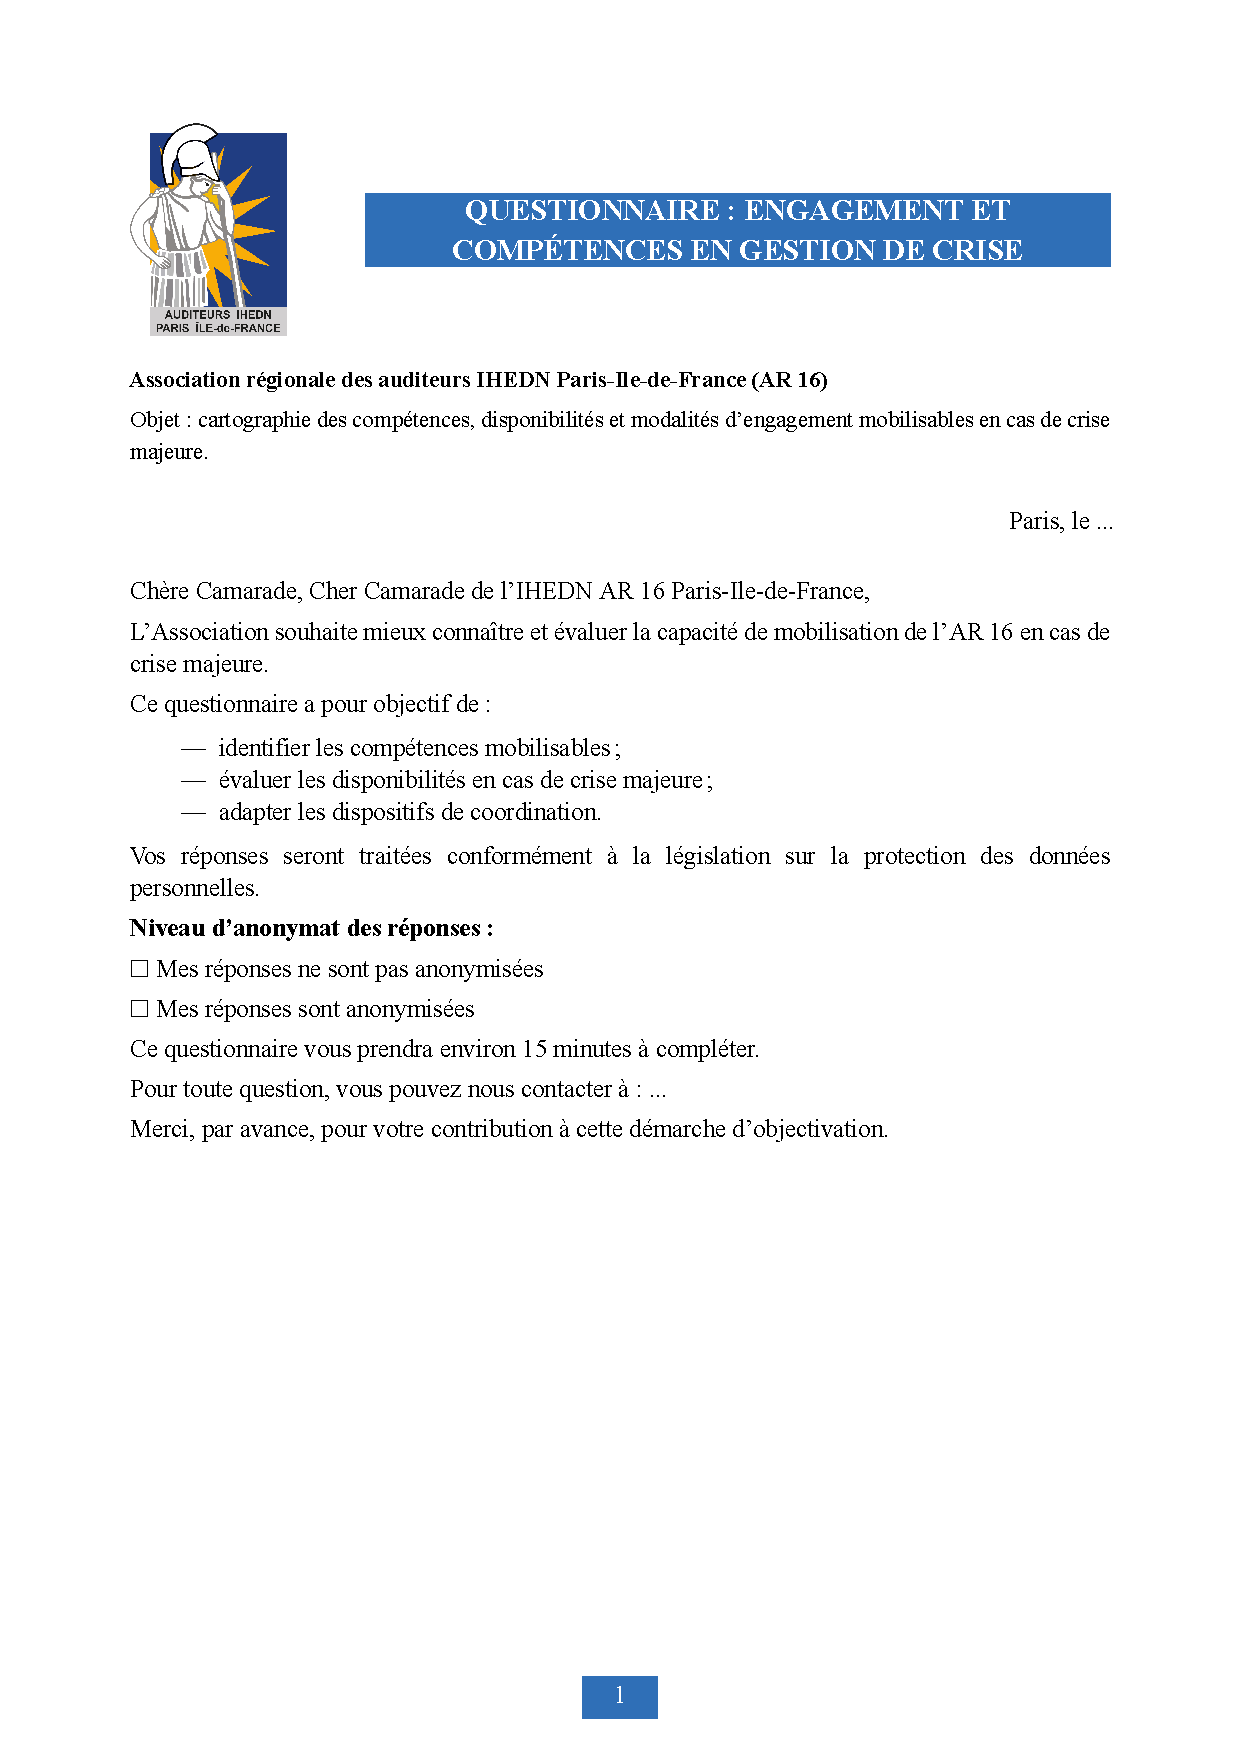
\includegraphics[page=1,width=0.84\textwidth]{QCM.pdf}
\end{tcolorbox}
\clearpage

\foreach \IhednIncludedPdfPage in {2,...,\the\IhednIncludedPdfPageCount}{%
  \begin{tcolorbox}[
    colback=gray!5,
    colframe=black,
    boxrule=0.5pt,
    arc=3mm
  ]
  \centering
  \includegraphics[page=\IhednIncludedPdfPage,width=0.95\textwidth]{QCM.pdf}
  \end{tcolorbox}
  \ifnum\IhednIncludedPdfPage<\IhednIncludedPdfPageCount
    \clearpage
  \fi
}%


\addcontentsline{toc}{section}{Références bibliographiques}
\printbibheading[title={Références bibliographiques}]

\addcontentsline{toc}{subsection}{Ouvrages}
\newrefcontext[sorting=nyt]
\printbibliography[	keyword=livre,
					title={Ouvrages},
					heading=subbibliography]

\addcontentsline{toc}{subsection}{Articles de recherche}
\newrefcontext[sorting=nyt]
\printbibliography[	keyword=article_de_recherche,
					title={Articles de recherche},
					heading=subbibliography]

\addcontentsline{toc}{subsection}{Rapports institutionnels}
\newrefcontext[sorting=nyt]
\printbibliography[	keyword=rapport_institutionnel,
					title={Rapports institutionnels},
					heading=subbibliography]

\addcontentsline{toc}{subsection}{Ressources en ligne}
\newrefcontext[sorting=nyt]
\printbibliography[	keyword=article_online,
					title={Ressources en ligne},
					heading=subbibliography]

\addcontentsline{toc}{subsection}{Articles de presse en ligne}
\newrefcontext[sorting=nyt]
\printbibliography[	keyword=article_presse_online,
					title={Articles de presse en ligne},
					heading=subbibliography]

\end{document}
